
\chapter{Simulation}
\label{chap:simulations}

This chapter presents the results obtained in simulation for the MPC problem of path planning according to the parameters and conditions mentioned in the chapter \ref{chap:controller_evaluation}. In an unrestricted scenario with no change in environmental conditions or road conditions.
\\
\\
For the simulation, the following assumptions are taken:
\begin{itemize}
    \item All vehicles have the same dimensions.
    \item All vehicles have the same dynamic model, and there is no difference between them.
    \item The highway environment has no curves or intersections.
    \item The target speed and the desired lane are adjusted according to the interest of each driver.
\end{itemize}

\\
\\
The figures shown below are from different times. The initial time step shows the desired location and trajectories when $t_0=0$. In the time step, it is possible to see the most difficult maneuver to perform for some of the network agents. Finally, it is possible to see that everyone achieves their goal at the end of the control solution.
\\
\\
Colored squares represent vehicles, and circles represent possible crash risk areas. Colored dotted lines represent the predicted trajectories according to the agent to which they correspond. A final plot will be shown with as much information as possible in order to interpret the movement that the vehicles would have in a real scenario.
\\
\\
The main simulations were carried out with N=12 vehicles. However, simulations were made to analyze computation time with N = {2, 10} vehicles. First, the three most essential times in the simulation are shown, and then the quality and feasibility of each of the controllers will be discussed. In decentralized and centralized controllers, the trajectories are similar because the intention is to have the same working conditions. After a centralized and decentralized controller simulation, it is presented an analytic analysis. The analysis is based on the computation time as a function of the number of vehicles, the time per iteration of each controller, the increment of the computation time as a function of the prediction horizon, and the total simulation time as a function of the number of vehicles connected to the net. At the end of each section, a conclusion of each scenario will be given.
\\
\\
The solution algorithm is solved in MATLAB \cite{Matlab}. OCPs are solved using the GUROBI mathematical optimization engine with the YALMIP programming interface. GUROBI optimization engine is chosen to solve most problems due to its powerful branch and bound algorithm. With this, it is possible to solve mixed-integer quadratic programming problems (MIQP) in the presence of non-linear models. This section of the document seeks to evaluate the behavior of vehicles in a selfish environment dealing with selfish agents and trying to reach their goal. 


\section{Unrestricted Scenario.}

The unrestricted scenario is designed with 12 vehicles on the same road. It also has six lanes in line, and the road is one-way. There are no intersections, traffic lights, obstacles, crossings, or any obstructions in the simulation environment.


\begin{figure}[h!]
\centering
\begin{subfigure}[t]{\textwidth}
    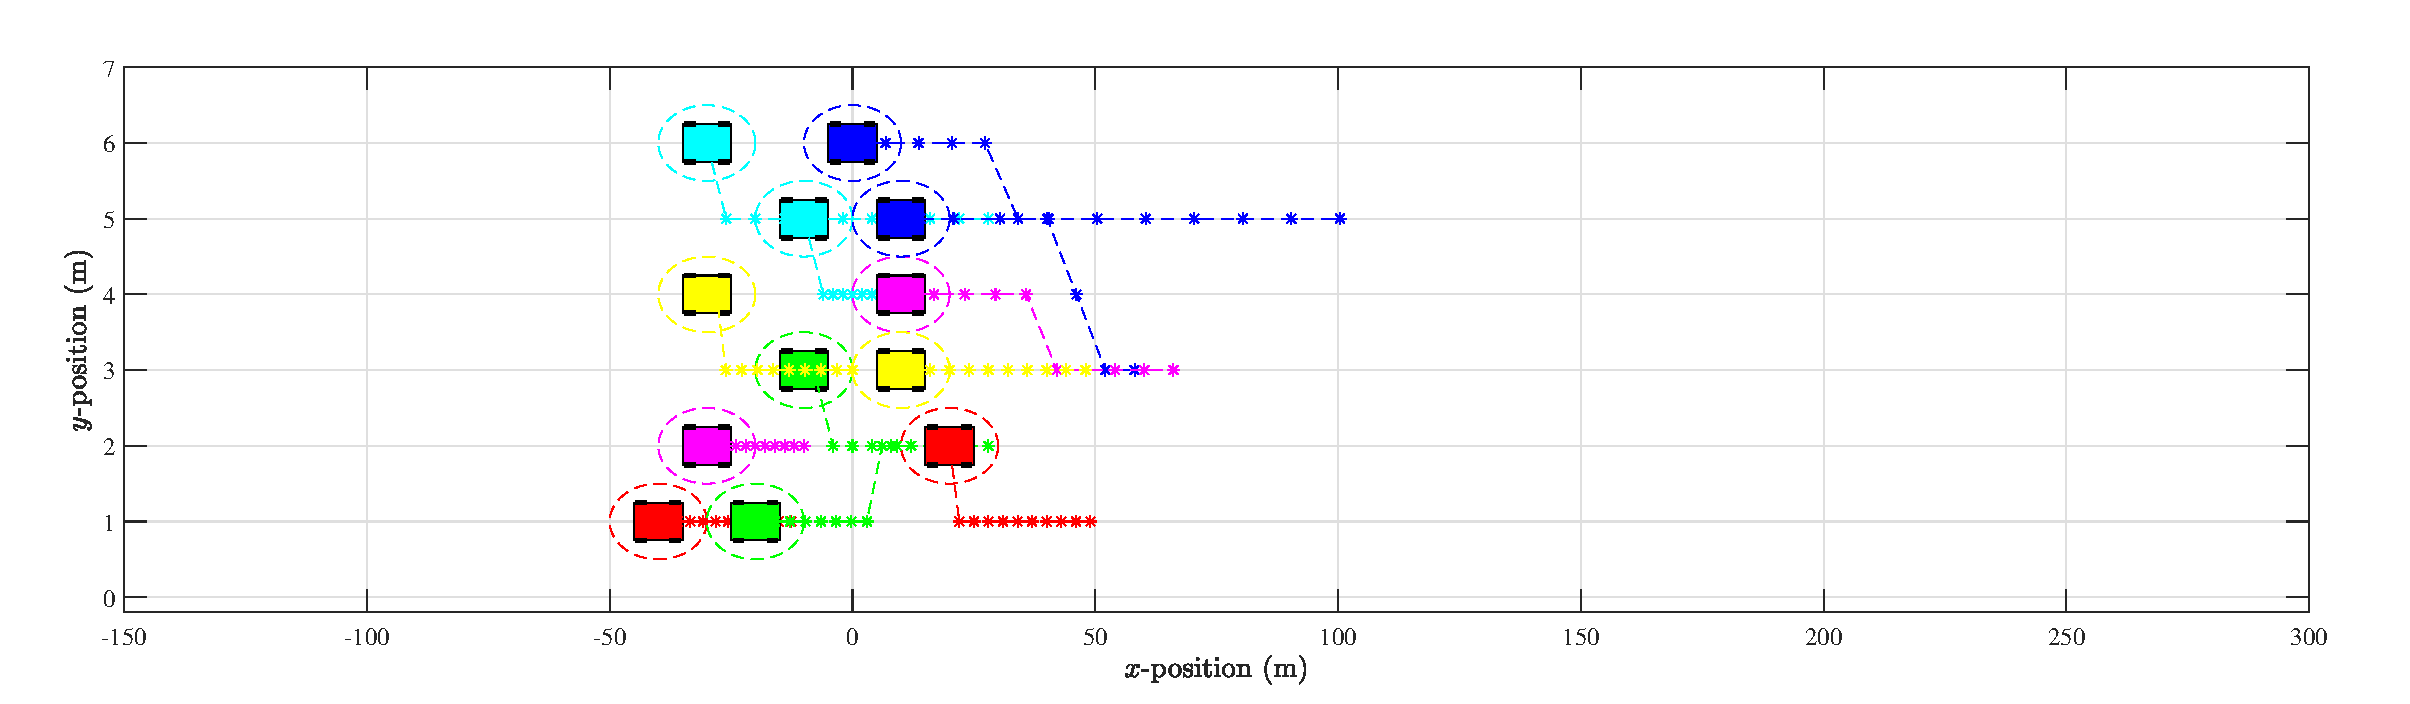
\includegraphics[width=\textwidth]{Kap6/no_restricted/no_restricted_traj0.eps}
    % \caption{Predicted positions.}
    \label{fig:first}
\end{subfigure}
\vspace{1cm}
\begin{subfigure}[b]{0.45\textwidth}
    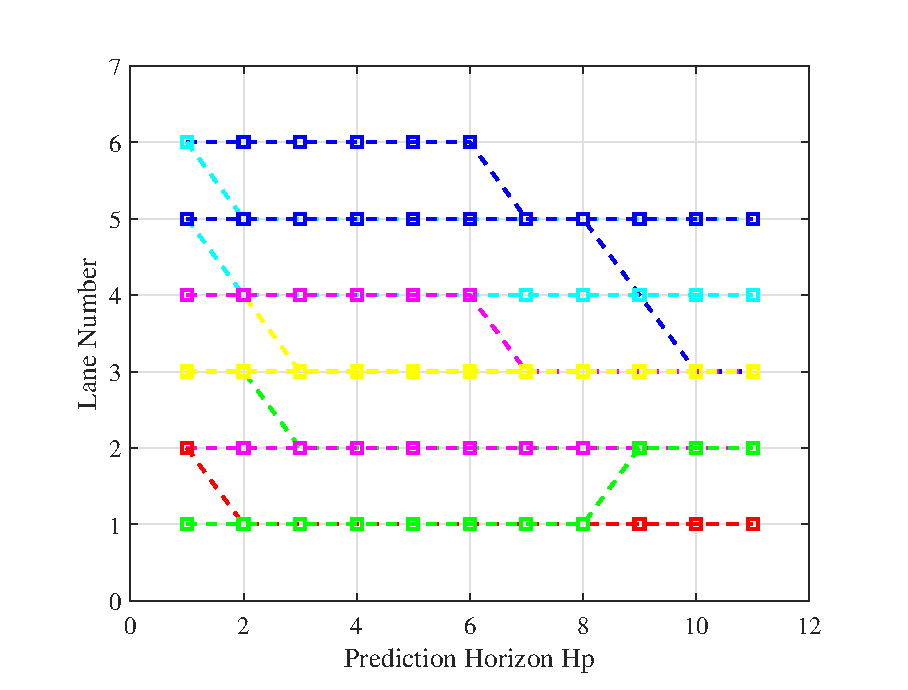
\includegraphics[width=\textwidth]{Kap6/no_restricted/no_restricted_lane0.eps}
    % \caption{Predicted lane profiles.}
    \label{fig:second}
\end{subfigure}
\hfill
\begin{subfigure}[b]{0.45\textwidth}
    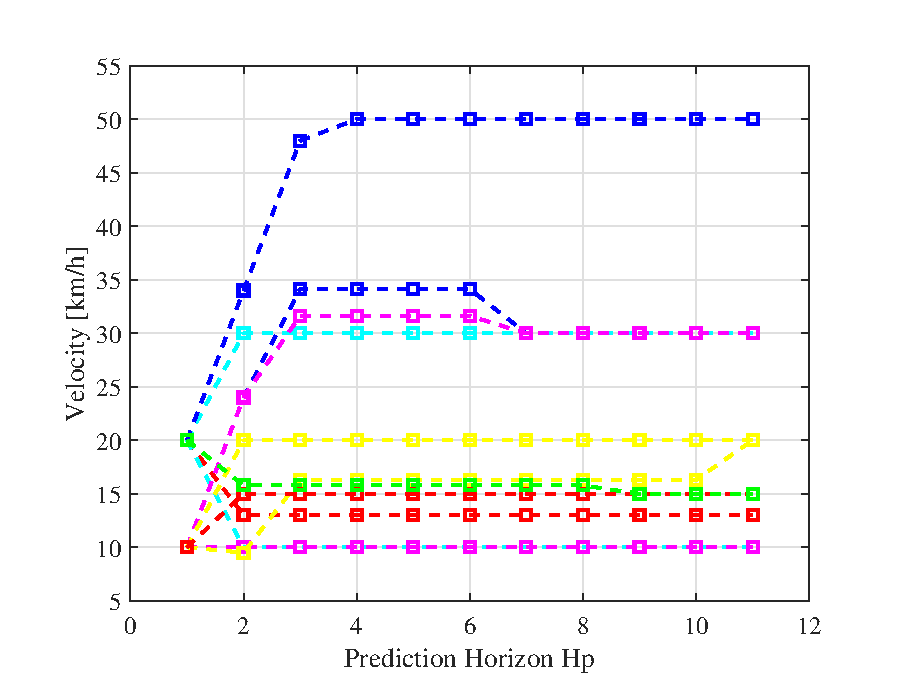
\includegraphics[width=\textwidth]{Kap6/no_restricted/no_restricted_vel0.eps}
    % \caption{Predicted velocity profiles.}
    \label{fig:third}
\end{subfigure}
\caption{MPC Iteration = 0. Initial conditions}
\label{fig:figures}
\end{figure}

\vspace{0.5cm}
At the beginning of the simulation, the vehicles are adjusted to an initial position and speed, as explained in more detail in the \ref{subsec:descentr} chapter. As seen in the image in the first step, each of the agents has a predicted trajectory taking into account the predicted trajectories of its neighbors.


% /////////////////////////////////////////////////
% ..........................................
\begin{figure}[h!]
\centering
\begin{subfigure}[t]{\textwidth}
    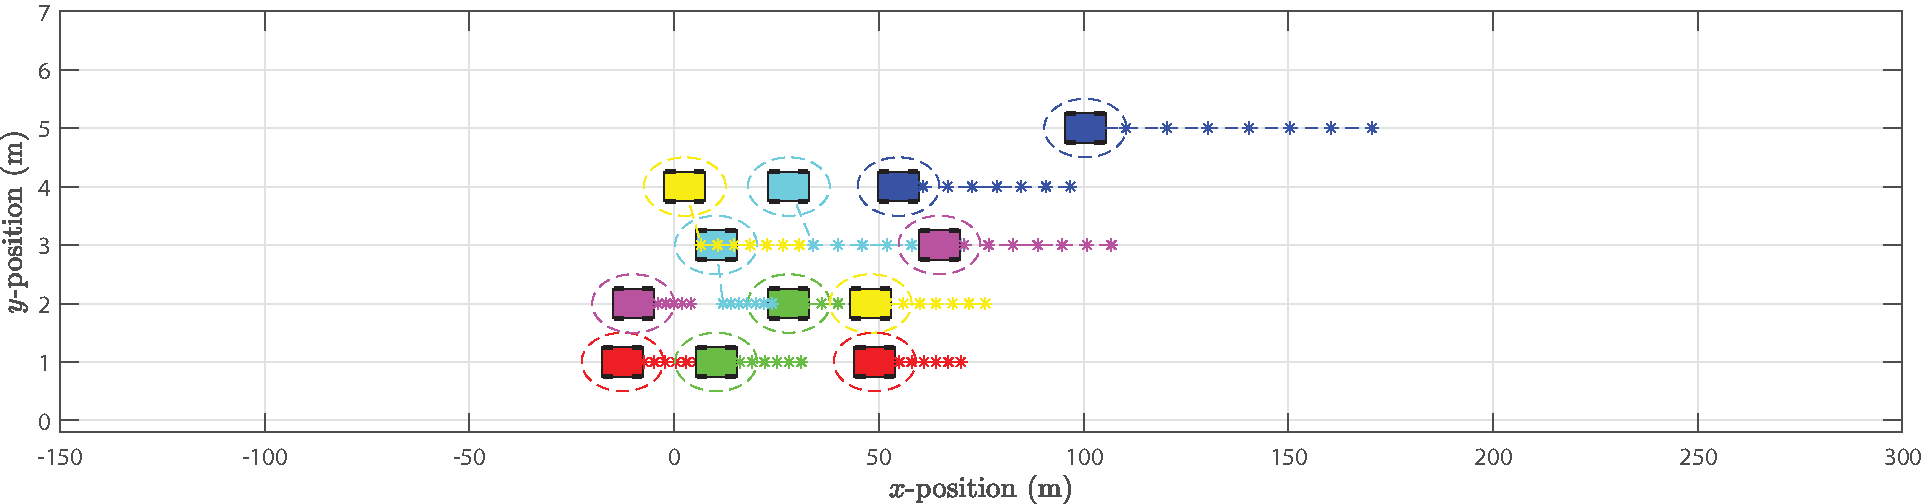
\includegraphics[width=\textwidth]{Kap6/no_restricted/no_restricted_traj10.eps}
    \caption{Predicted position.}
    \label{fig:first}
\end{subfigure}
\vspace{1cm}
\begin{subfigure}[b]{0.45\textwidth}
    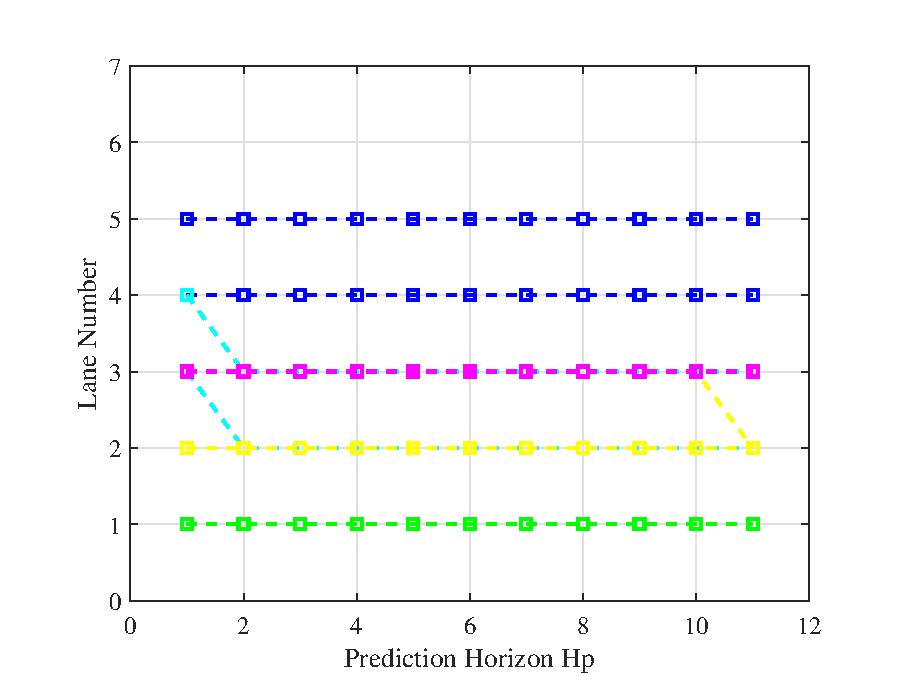
\includegraphics[width=\textwidth]{Kap6/no_restricted/no_restricted_lane10.eps}
    \caption{Predicted lane positions.}
    \label{fig:second}
\end{subfigure}
\hfill
\begin{subfigure}[b]{0.45\textwidth}
    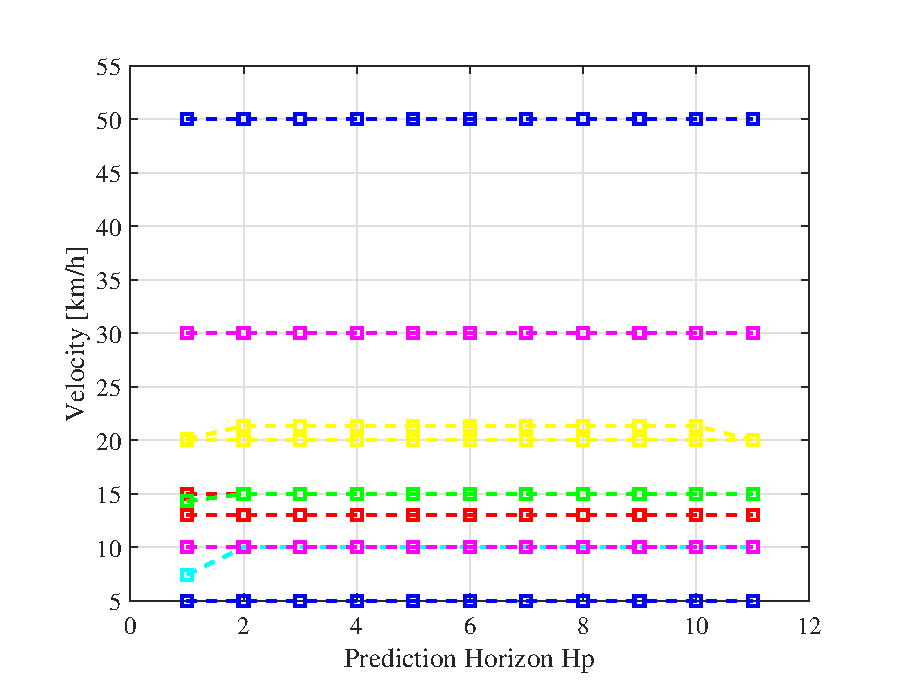
\includegraphics[width=\textwidth]{Kap6/no_restricted/no_restricted_vel10.eps}
    \caption{Predicted velocity profiles.}
    \label{fig:third}
\end{subfigure}
\caption{MPC Iteration = 10. Vh 2,3,4,6 change lanes.}
\label{fig:figures}
\end{figure}

In the first scenario, the centralized and decentralized controllers achieve the main objective of each of the agents. The trajectories travelled during the simulation time in both cases are the same because the initial conditions and the main objective are the same. Therefore, the paths shown are equivalent for both network architectures.

% .........................................
\begin{figure}[H]
\centering
\begin{subfigure}[t]{\textwidth}
    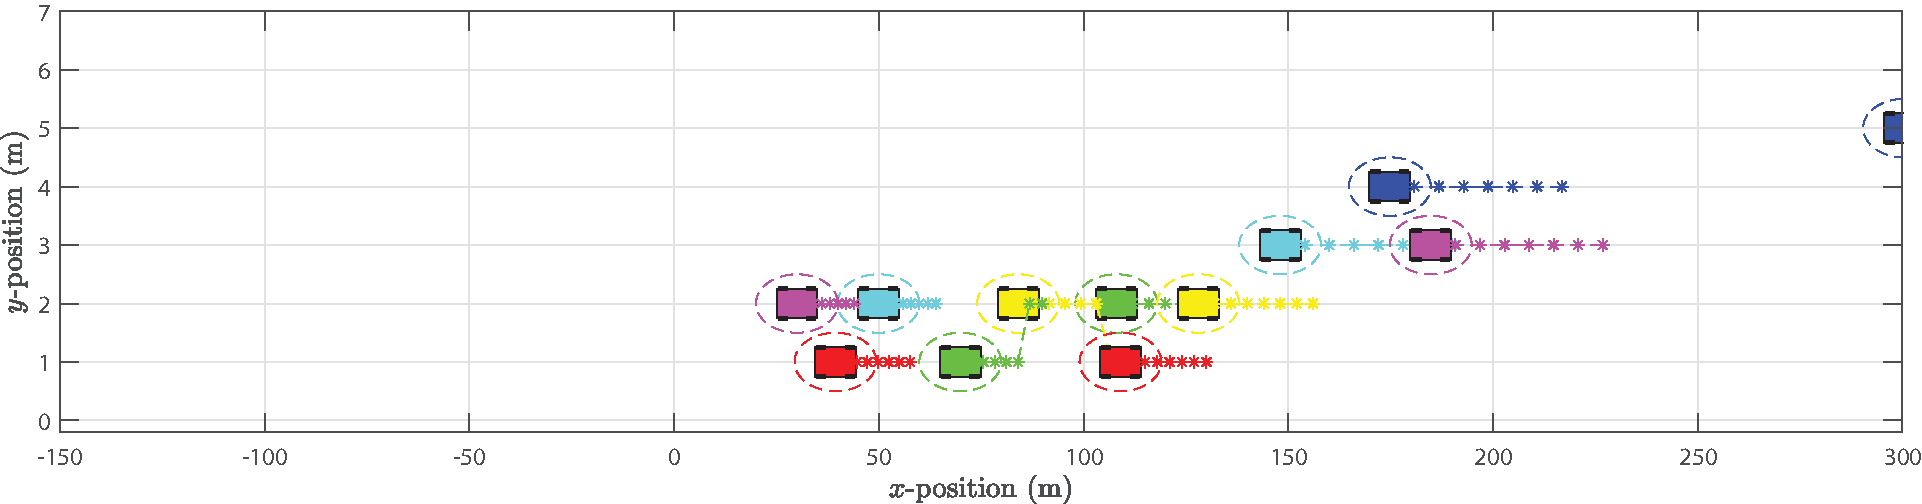
\includegraphics[width=\textwidth]{Kap6/no_restricted/no_restricted_traj30.eps}
    \caption{Predicted position at first position.}
    \label{fig:first}
\end{subfigure}
\vspace{1cm}
\begin{subfigure}[b]{0.45\textwidth}
    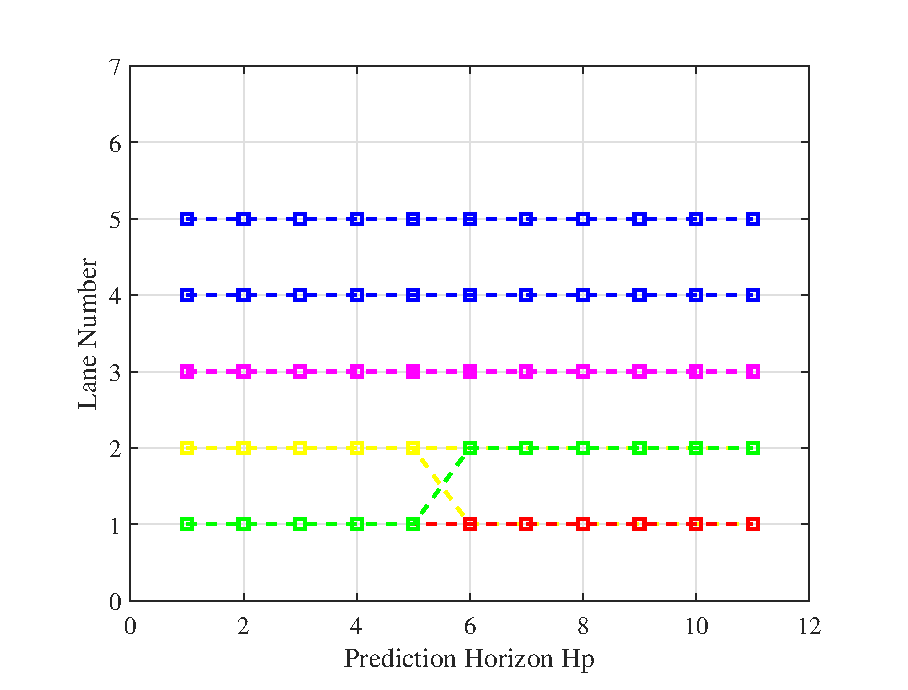
\includegraphics[width=\textwidth]{Kap6/no_restricted/no_restricted_lane30.eps}
    \caption{Predicted lane positions.}
    \label{fig:second}
\end{subfigure}
\hfill
\begin{subfigure}[b]{0.45\textwidth}
    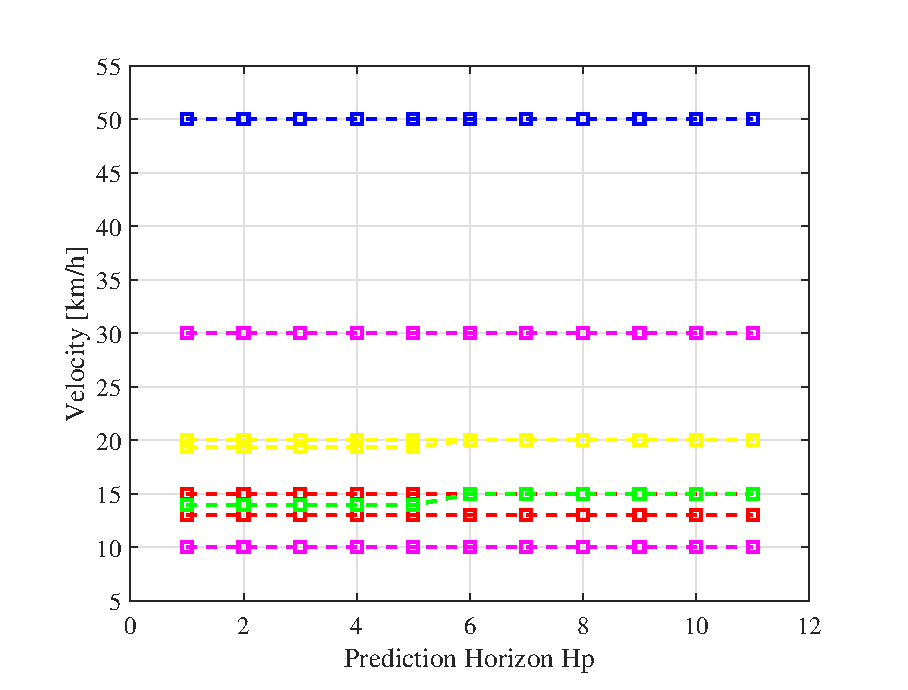
\includegraphics[width=\textwidth]{Kap6/no_restricted/no_restricted_vel30.eps}
    \caption{Predicted velocity profiles.}
    \label{fig:third}
\end{subfigure}
\caption{MPC Iteration = 30. The overall goal of the network is achieved }
\label{fig:figures}
\end{figure}
% .......................................

\\

\begin{figure}[H]
\centering
    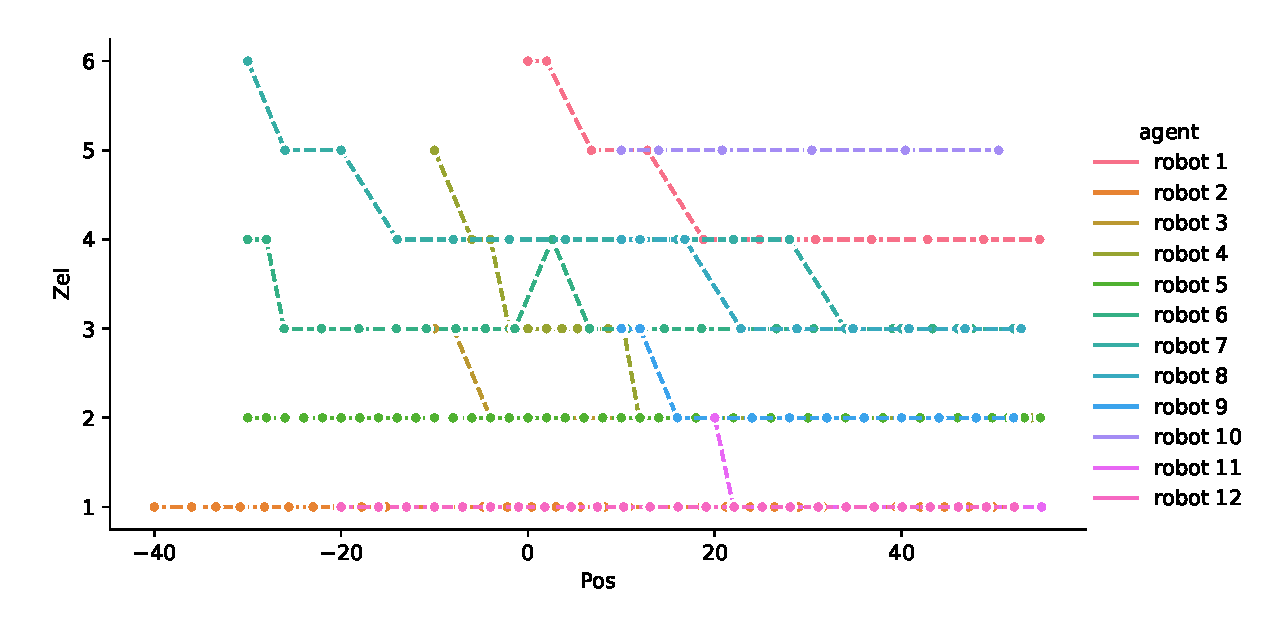
\includegraphics[width=0.8\textwidth]{Kap6/no_restricted/no_restricted_trajectories.eps}
    \caption{Trajectories of the entire network during the simulation time.}
\end{figure}

% ////////////////////////////



\\

% \subsection{Computation Time}
\vspace{0.5cm}
The computation time of D-MPC during the entire simulation is computed with the mean of each step sample. In Fig \ref{Step_time_no_rest}, it can see the average time that the network takes to solve each step $k$ of the solution algorithm. In addition, the time taken by the fastest controller (lower barrier) and the slower controller (upper barrier) is shown. The time it takes for each agent to resolve its OCP depends on the environmental conditions and the main objective it is looking for.
\\
\begin{figure}[H]
\centering
    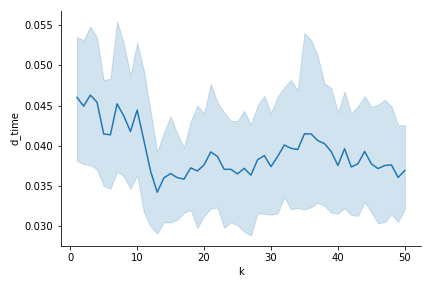
\includegraphics[width=.6\textwidth]{Kap6/no_restricted/no_restricted_d_time.png}
    \caption{Step time}
        \label{Step_time_no_rest}
\end{figure}

% ...........................



\begin{figure}[h!]
\centering
    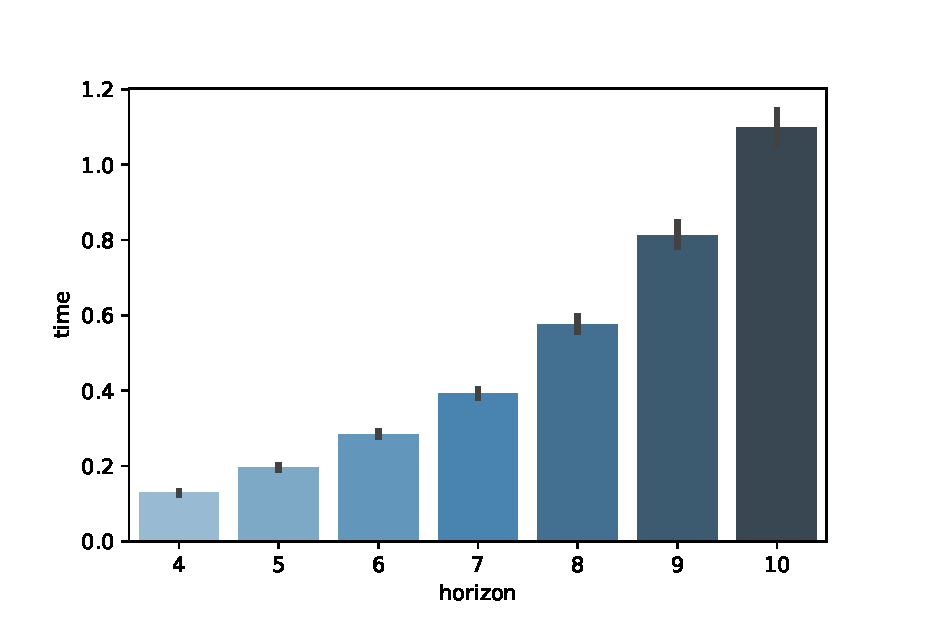
\includegraphics[width=0.6\textwidth]{Kap6/no_restricted/no_restricted_horizon_time.eps}
    \caption{Non-linear model of a differential robot.}
    % \label{kinematic2}
\end{figure}

Finally, an analysis of the time difference in the architectures is made. It is remarkable to see the improvement of the D-MPC networks. However, for real-time driving, the solution time is not enough.

\begin{figure}[H]
\centering
    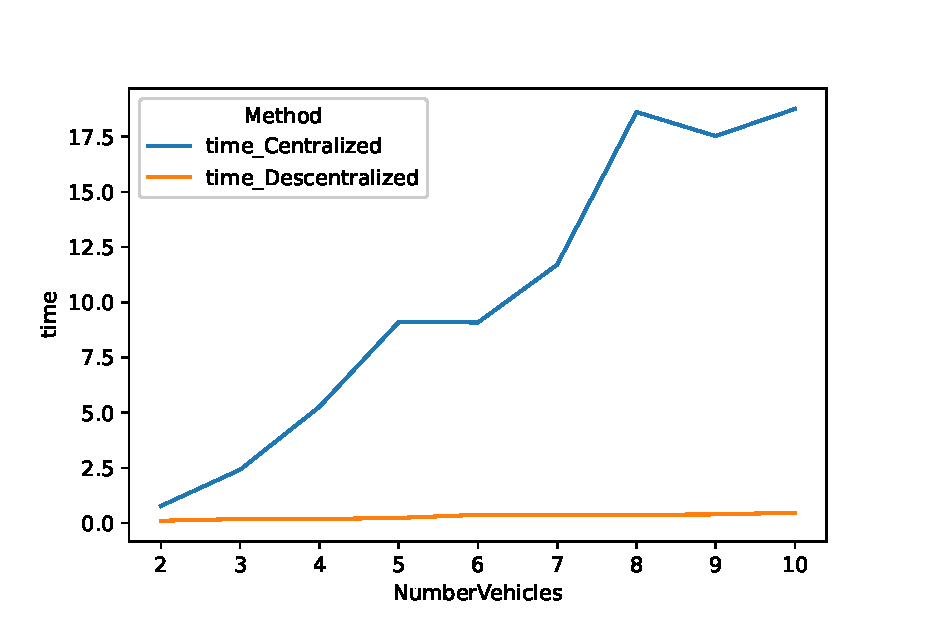
\includegraphics[width=0.6\textwidth]{Kap6/no_restricted/no_restricted_n_vehicles.eps}
    \caption{Computation time vs Number of vehicles.}
    % \label{kinematic2}
\end{figure}



% % ...........................
% \subsubsection{Trajectory Quality}

% ...........................
% \subsubsection{Controller Comparison - Unrestricted scenario}

% ...........................
\subsubsection{Conclusion Unrestricted Scenario}

Both control structures (C-MPC and D-MPC) show that autonomous driving is possible in a highway environment. The Potential game's framework allows the controller to take into account the conditions of others and make the optimal decisions in selfish scenarios.
\\
\\
Given the time results, it can be concluded that in a highway scenario, it is not possible to drive a vehicle with this technique due to the lack of computing power that we currently have to be able to solve this problem in a specific time. Solution times in D-MPC are much lower than what is seen in C-MPC. The C-MPC manages to give an optimal solution, but its solution takes a long time. Also, sometimes the controller falls into local minimums but fails to reach a global minimum.

\newpage
% -------------------------------------------
\section{Obstacle Avoidance Scenario}
% -------------------------------------------

The obstacle avoidance scenario was designed with 12 vehicles on the same road. It also has six lanes in line, and the road is one-way. There is one vehicle in the lane $L=3$  with no movement. It represents an obstacle that the controller's vision system could recognize. The main objective is to prevent the damaged vehicle from achieving its objective speed and lane.

\begin{figure}[H]
\centering
\begin{subfigure}[t]{\textwidth}
    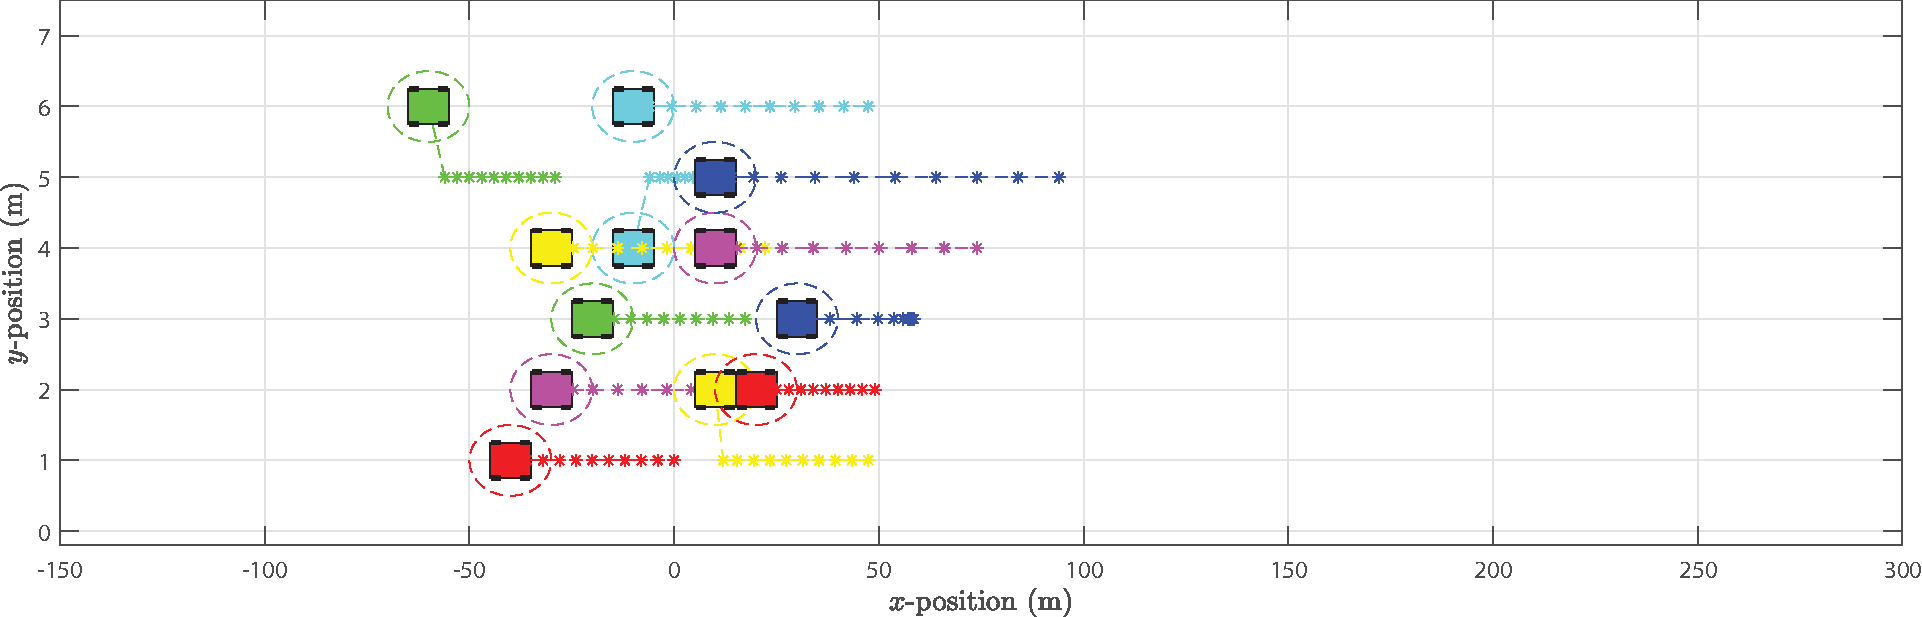
\includegraphics[width=\textwidth]{Kap6/obs_avoid/obs_avoid_traj0.eps}
    \caption{Predicted positions.}
    \label{fig:first}
\end{subfigure}
\vspace{1cm}
\begin{subfigure}[b]{0.45\textwidth}
    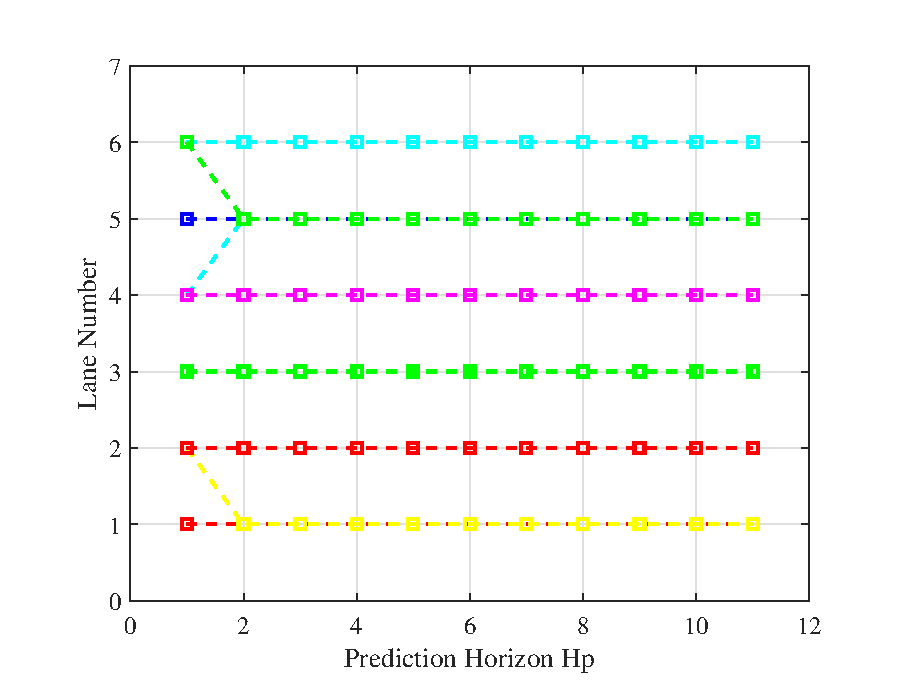
\includegraphics[width=\textwidth]{Kap6/obs_avoid/obs_avoid_lane0.eps}
    \caption{Predicted lane profiles.}
    \label{fig:second}
\end{subfigure}
\hfill
\begin{subfigure}[b]{0.45\textwidth}
    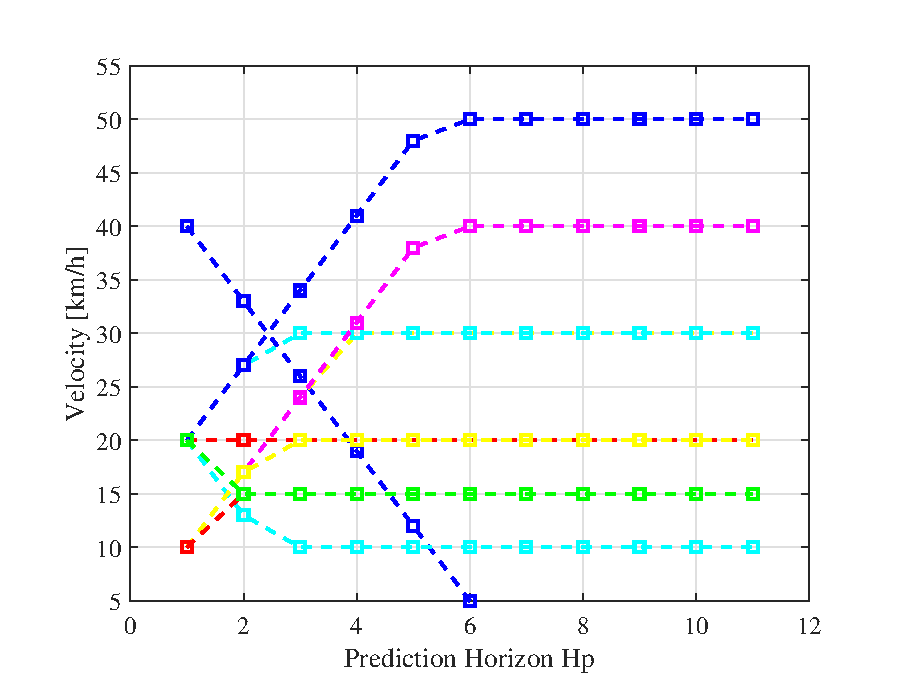
\includegraphics[width=\textwidth]{Kap6/obs_avoid/obs_avoid_vel0.eps}
    \caption{Predicted velocity profiles.}
    \label{fig:third}
\end{subfigure}
\caption{MPC Iteration = 0.}
\label{fig:figures}
\end{figure}

In iteration 0, the controller adjusts the initial positions of all the vehicles and the initial conditions. The scenario poses a vehicle blocked on the road so that the vehicle detection system can detect this new obstacle. It is essential to mention that in the first step, three vehicles are planning in their path plans to change lanes. Those are the only vehicles that can change lanes. In addition, the rest of the neighbors do not plan to change lanes because they have vehicles around them.
\\

% ........................................
\begin{figure}[H]
\centering
\begin{subfigure}[t]{\textwidth}
    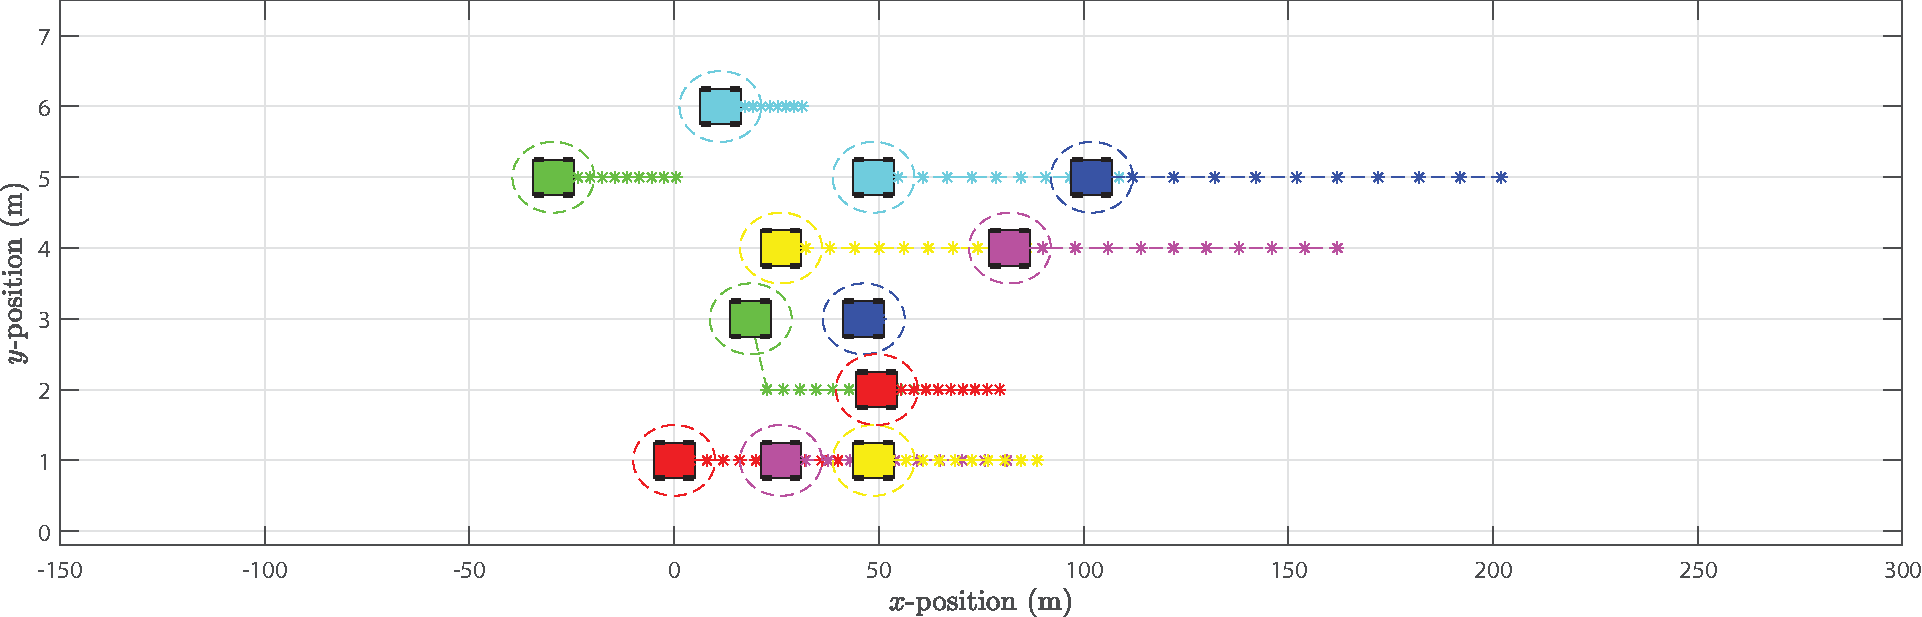
\includegraphics[width=\textwidth]{Kap6/obs_avoid/obs_avoid_traj20.eps}
    \caption{Predicted position.}
    \label{fig:first_mpc10}
\end{subfigure}
\vspace{1cm}
\begin{subfigure}[b]{0.45\textwidth}
    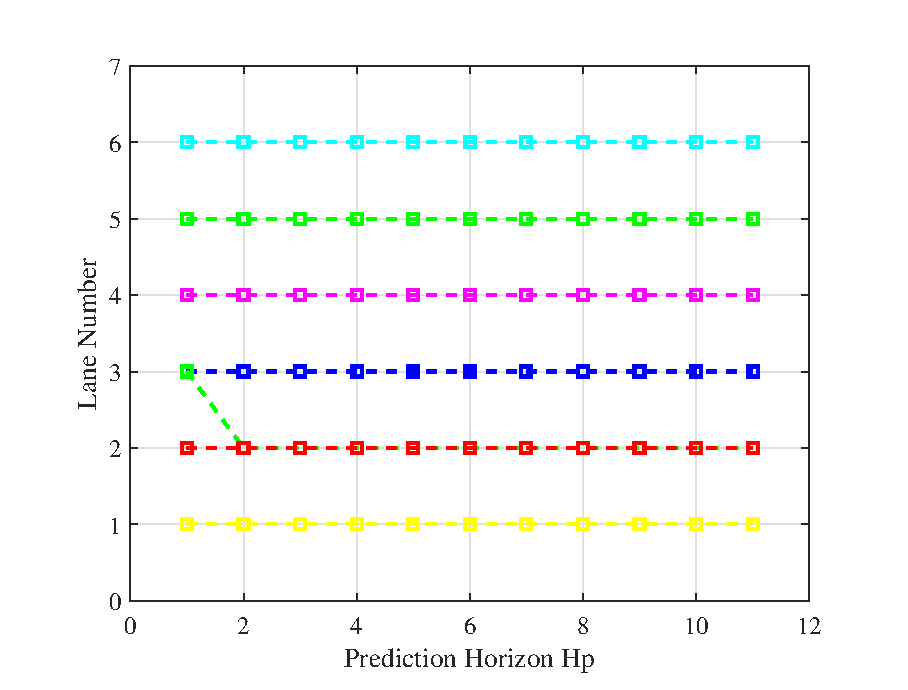
\includegraphics[width=\textwidth]{Kap6/obs_avoid/obs_avoid_lane20.eps}
    \caption{Predicted lane positions.}
    \label{fig:second_mpc10_obsav}
\end{subfigure}
\hfill
\begin{subfigure}[b]{0.45\textwidth}
    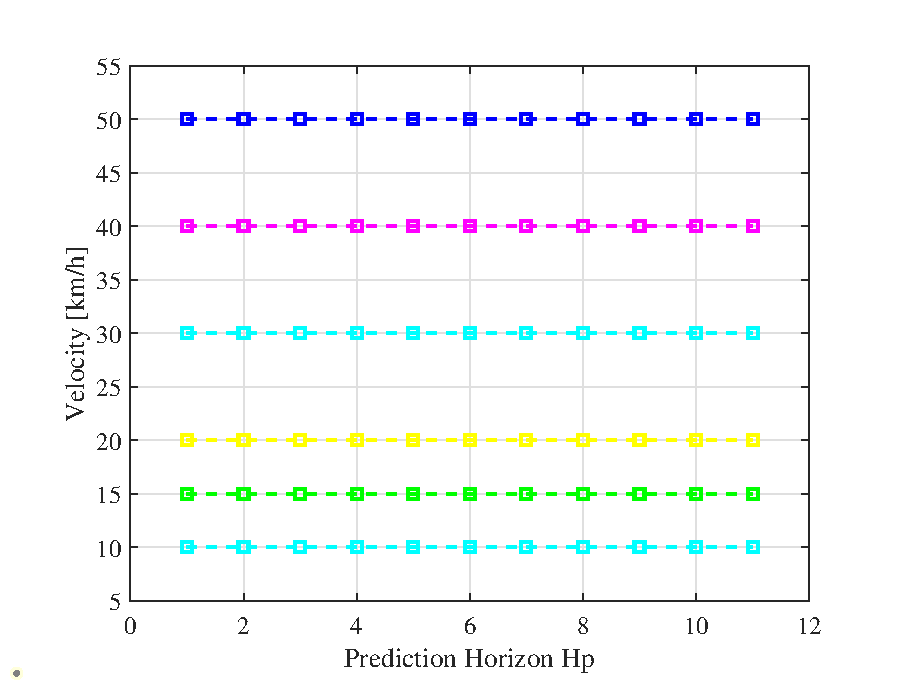
\includegraphics[width=\textwidth]{Kap6/obs_avoid/obs_avoid_vel20.eps}
    \caption{Predicted velocity profiles.}
    \label{fig:third}
\end{subfigure}
\label{fig:obs_mpc10}
\caption{MPC Iteration = 10.}
\end{figure}



In fig \ref{fig:first_mpc10}, it is possible to notice how vehicle number 3 (green color) has a trajectory prediction avoiding the obstacle. In addition, the other vehicles have changed lanes avoiding the obstacle. The vehicles $\mathcal{V}= \left\{ 4,2,5 \right\}$ (color red, purple, yellow) have already reached their desired lane without colliding with the others. In fig \ref{fig:second_mpc10_obsav}, the vehicles are not planning to change lanes because the majority have achieved their lane goal.

% .........................................
\begin{figure}[H]
\centering
\begin{subfigure}[t]{\textwidth}
    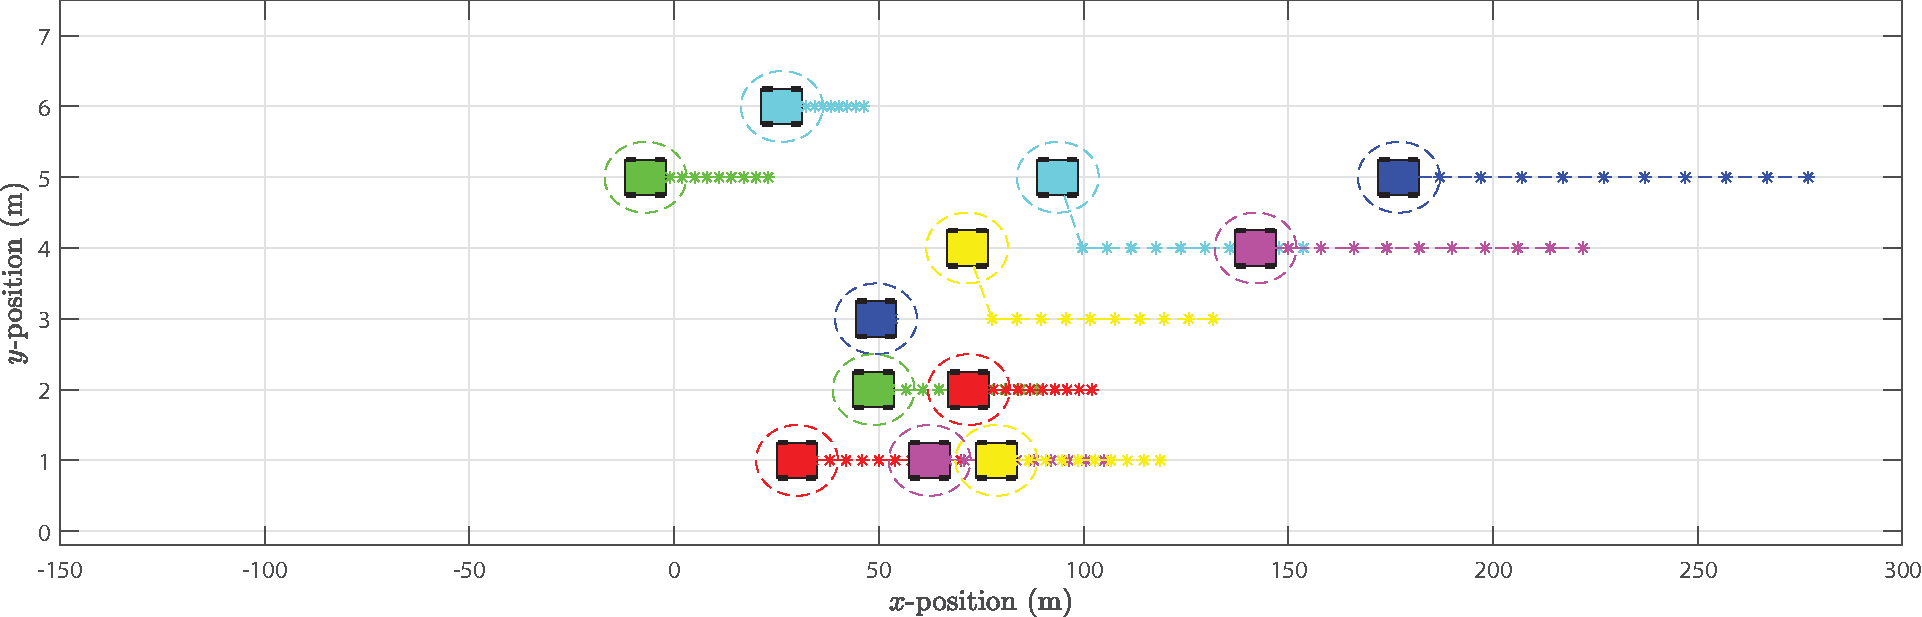
\includegraphics[width=\textwidth]{Kap6/obs_avoid/obs_avoid_traj40.eps}
    \caption{Predicted position at first position.}
    \label{fig:first}
\end{subfigure}
\vspace{1cm}
\begin{subfigure}[b]{0.45\textwidth}
    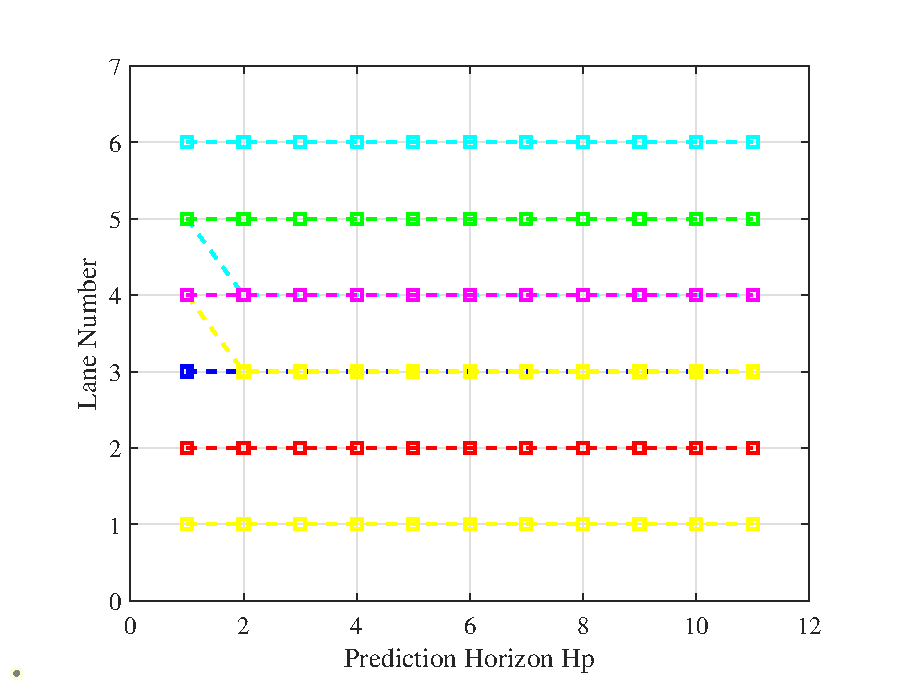
\includegraphics[width=\textwidth]{Kap6/obs_avoid/obs_avoid_lane40.eps}
    \caption{Predicted lane positions.}
    \label{fig:second}
\end{subfigure}
\hfill
\begin{subfigure}[b]{0.45\textwidth}
    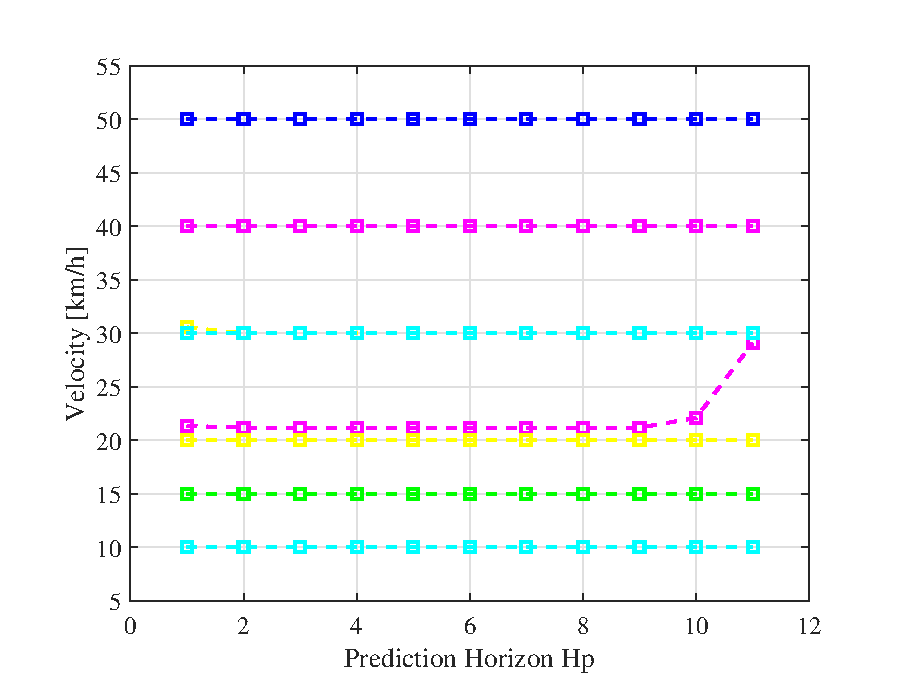
\includegraphics[width=\textwidth]{Kap6/obs_avoid/obs_avoid_vel40.eps}
    \caption{Predicted velocity profiles.}
    \label{fig:third}
\end{subfigure}
\caption{MPC Iteration = 30.}
\label{fig:figures}
\end{figure}
% .......................................
\begin{figure}[H]
\centering
    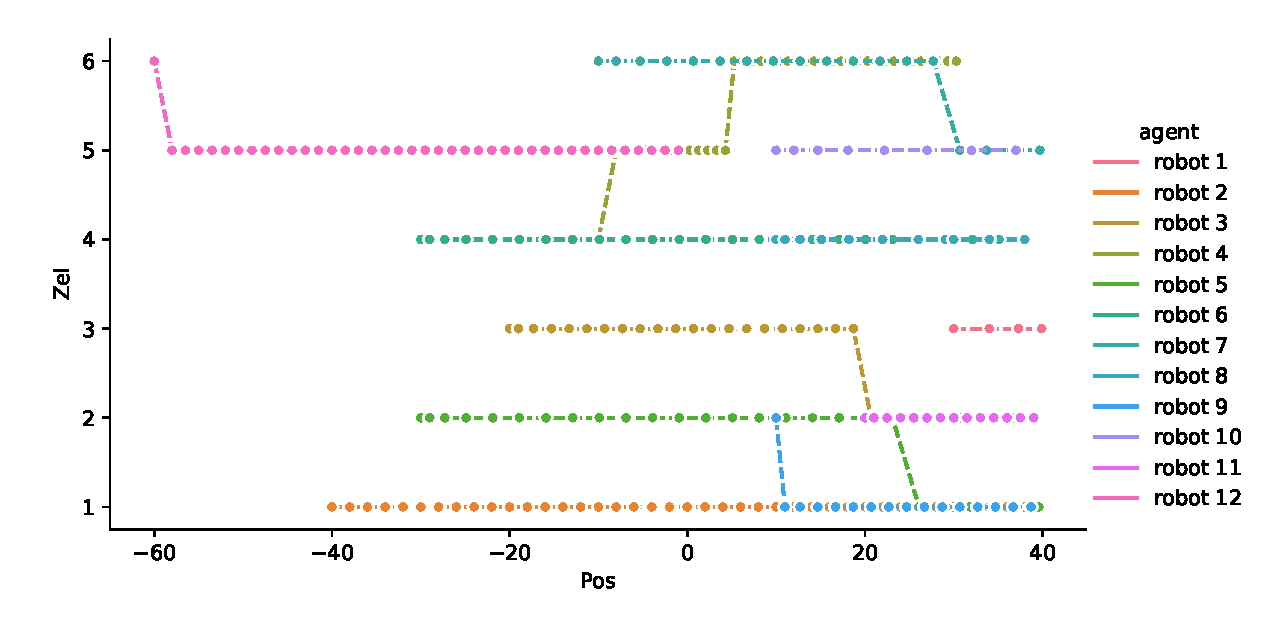
\includegraphics[width=0.8\textwidth]{Kap6/obs_avoid/obs_avoid_trajectories.eps}
    \caption{Trajectories of the entire network during the simulation time.}
\end{figure}

% ////////////////////////////


The simulation results show that the controller can provide a solution to obstacles that may arise Fig \ref{obs_avoid_step_time}. Also, the solution time of each of the sample steps is less in this scenario compared to the unconstrained scenario. This is due to the few interactions they have to do between vehicles after avoiding the obstacle vehicle. In addition, near step 10, it is possible to analyze the increase in solution time because in this step, the vehicles are dealing with the obstacle on the road.

\begin{figure}[H]
\centering
    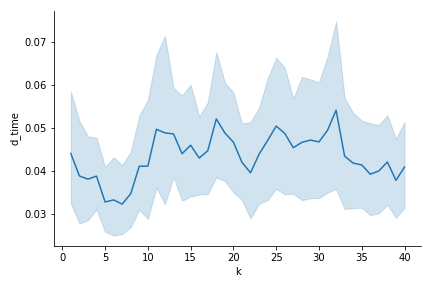
\includegraphics[width=.6\textwidth]{Kap6/obs_avoid/obs_avoid_d_time.png}
    \caption{Step Time}
    \label{obs_avoid_step_time}
\end{figure}

% ...........................

In the time analysis, depending on the prediction horizon, it can be seen that despite reaching 12 prediction steps, the system can provide a reasonable solution with a good time. In any case, the controller sometimes fails to find a minimum due to the big number of constraints.



\begin{figure}[H]
\centering
    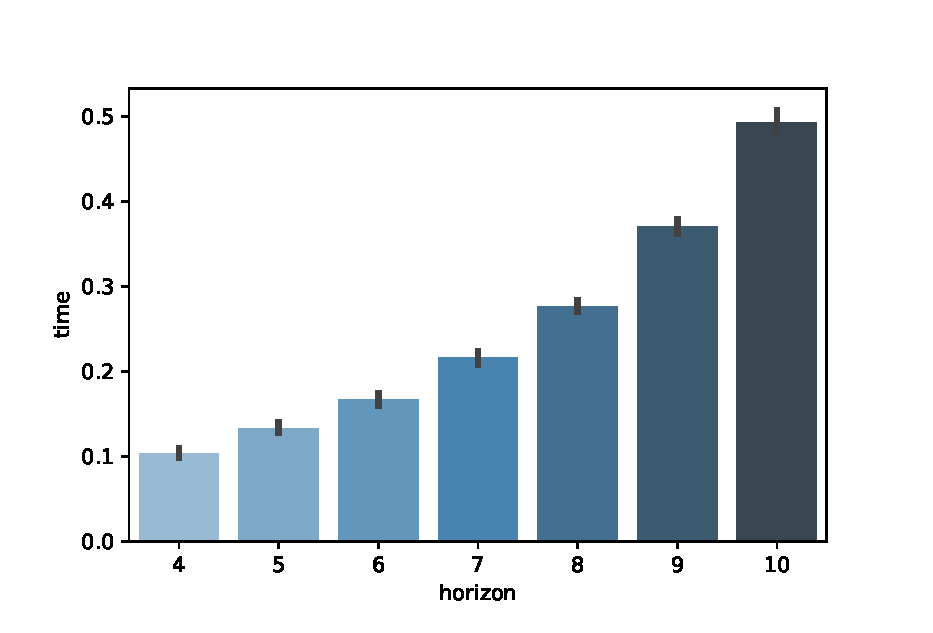
\includegraphics[width=0.6\textwidth]{Kap6/obs_avoid/obs_avoid_horizon_time.eps}
    \caption{Non-linear model of a differential robot.}
    % \label{kinematic2}
\end{figure}

Finally, as in the previous scenario, the difference in solving time is appreciated as the number of agents in the network increases. However, unlike the previous scenario, the D-MPC increases its duration with more vehicles.




\begin{figure}[H]
\centering
    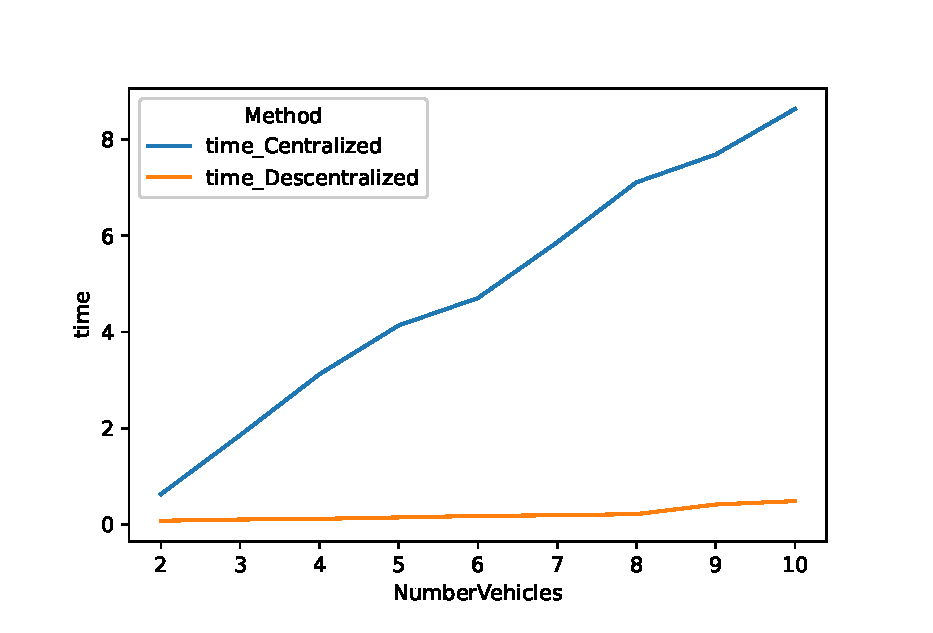
\includegraphics[width=0.6\textwidth]{Kap6/obs_avoid/obs_avoid_n_vehicles.eps}

\end{figure}


\subsection{Conclusion Obstacle Avoidance Scenario}

In a real highway environment, if a vehicle or other obstacle appears on the road, the decisions made by other vehicles are crucial. For this reason, this scenario of obstacles on the road was analyzed. With this new scenario, the number of constraints and the number of communications that each of the vehicles must deal with is greater than usual.

\\
\\
The obstacle avoidance scenario simulation shows that both C-MPC and D-MPC manage to solve the autonomous driving problem despite the increase in its constraints and a significant increase in communications between vehicles for the D-MPC case. However, the C-MPC continues to have difficulties providing an optimal solution in many evaluation cases. The system fell into an infeasible position causing the entire network to crash. This is because the solution algorithm that is used by the optimization engine (branch and bound) solves the problem by trying multiple possible solutions. While this is powerful, it can also be marginally unstable. The D-MPC manages to deal with the increase in constraints properly. However, more than the solution time is needed to be able to be implemented in real-time.

% \subsection{}

\newpage
% -------------------------------------------
\section{Reduced Scenario}
% -------------------------------------------

The reduced avoidance scenario was designed with 12 vehicles on the same road. It also has six lanes in line, and the road is one-way. There is a reduction in the number of lanes from 6 to 1. At a distance of 150 cm, the change starts. The main objective is to emulate a scenario where construction or change of the highway could happen. Moreover, it is an excellent opportunity to test the controller's behavior in the presence of a drastic change in its solution space. 

\begin{figure}[H]
\centering
\begin{subfigure}[t]{\textwidth}
    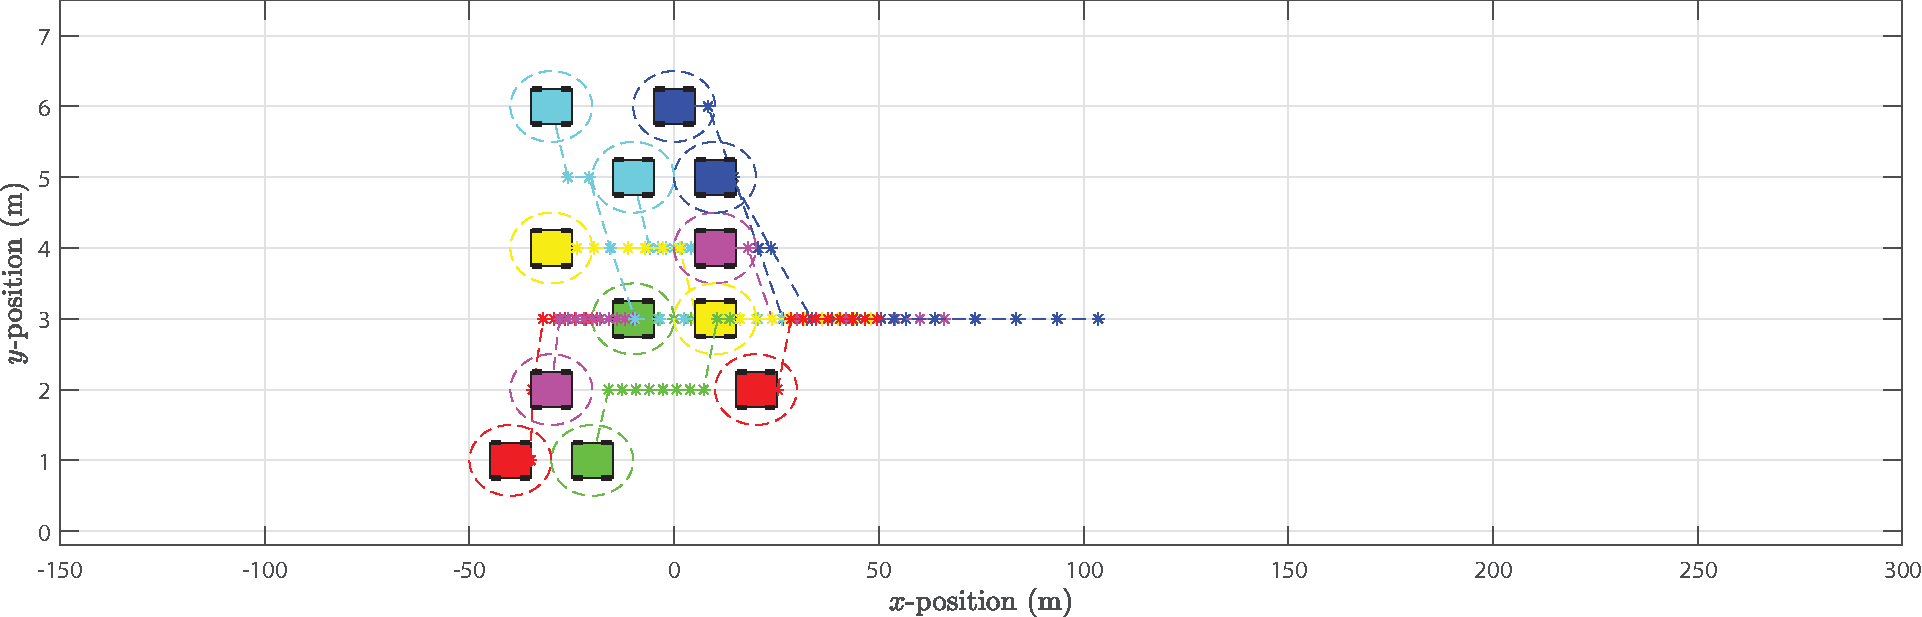
\includegraphics[width=\textwidth]{Kap6/red_lane/red_lane_traj0.eps}
    \caption{Predicted positions.}
    \label{fig:first}
\end{subfigure}
\vspace{1cm}
\begin{subfigure}[b]{0.45\textwidth}
    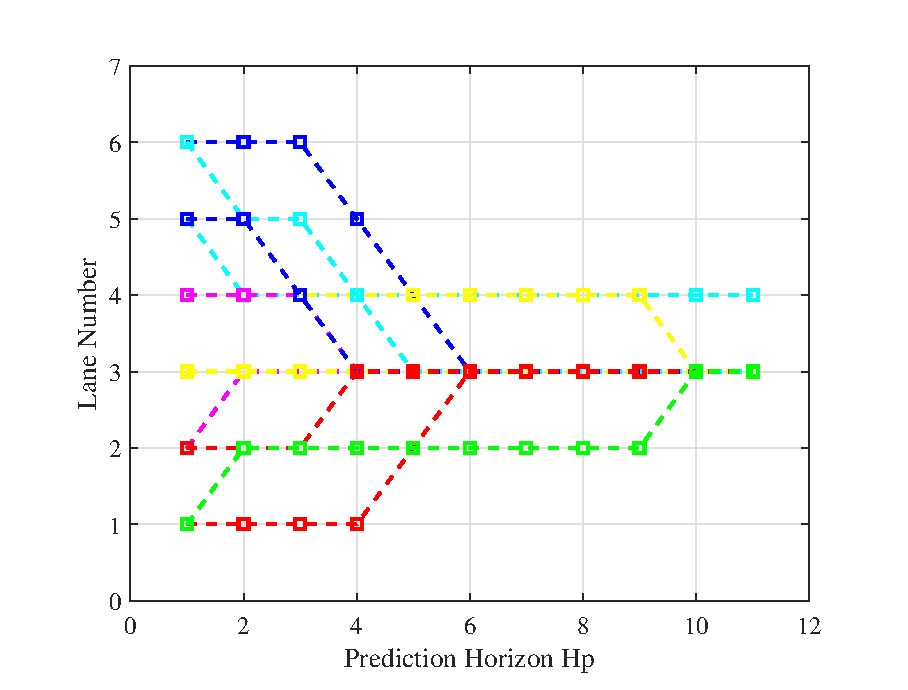
\includegraphics[width=\textwidth]{Kap6/red_lane/red_lane_lane0.eps}
    \caption{Predicted lane profiles.}
    \label{fig:second}
\end{subfigure}
\hfill
\begin{subfigure}[b]{0.45\textwidth}
    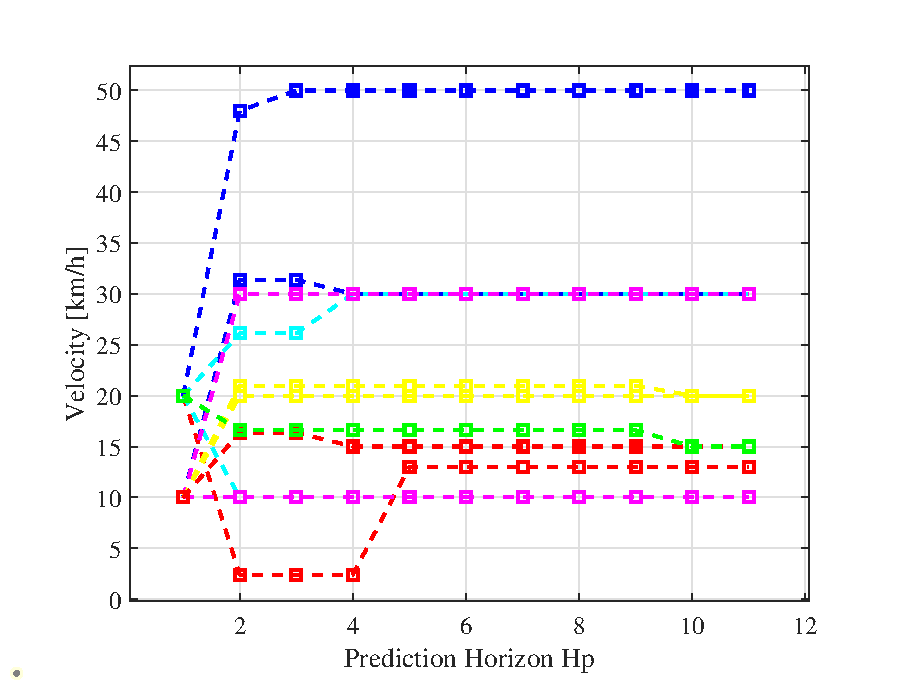
\includegraphics[width=\textwidth]{Kap6/red_lane/red_lane_vel0.eps}
    \caption{Predicted velocity profiles.}
    \label{fig:third}
\end{subfigure}
\caption{MPC Iteration = 0. Lane reduction scenario}
\label{fig:figures}
\end{figure}
\\
% ?.......................................
\begin{figure}[H]
\centering
\begin{subfigure}[t]{\textwidth}
    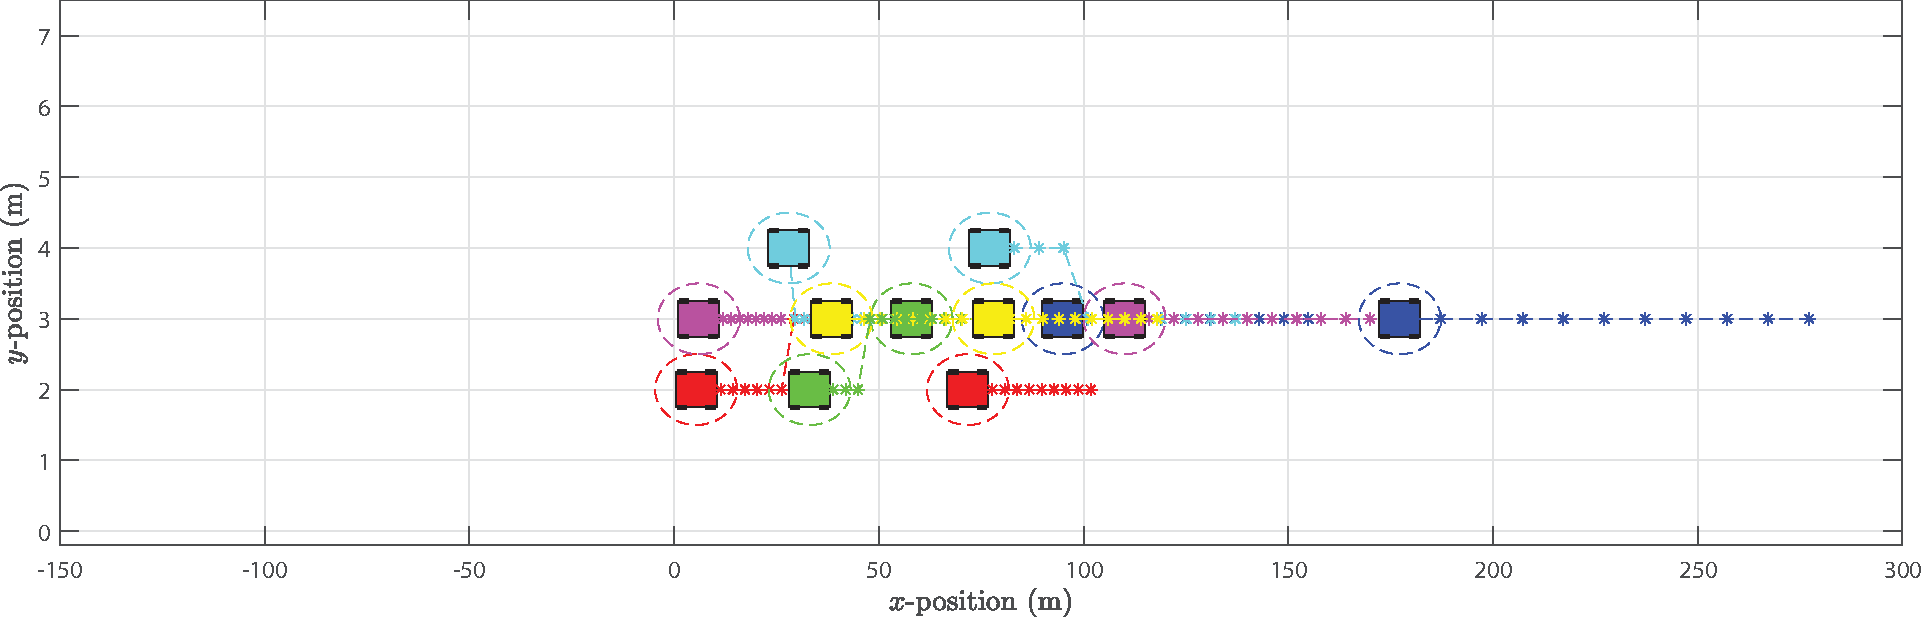
\includegraphics[width=\textwidth]{Kap6/red_lane/red_lane_traj10.eps}
    \caption{Predicted position.}
    \label{fig:first_mpc10_redsce}
\end{subfigure}
\vspace{1cm}
\begin{subfigure}[b]{0.45\textwidth}
    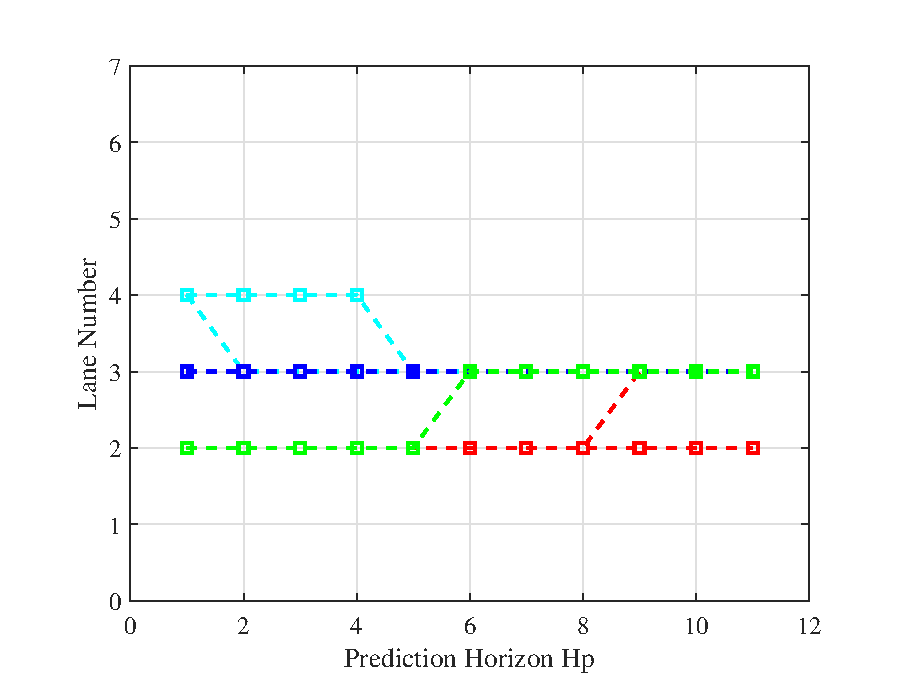
\includegraphics[width=\textwidth]{Kap6/red_lane/red_lane_lane10.eps}
    \caption{Predicted lane positions.}
    \label{fig:second}
\end{subfigure}
\hfill
\begin{subfigure}[b]{0.45\textwidth}
    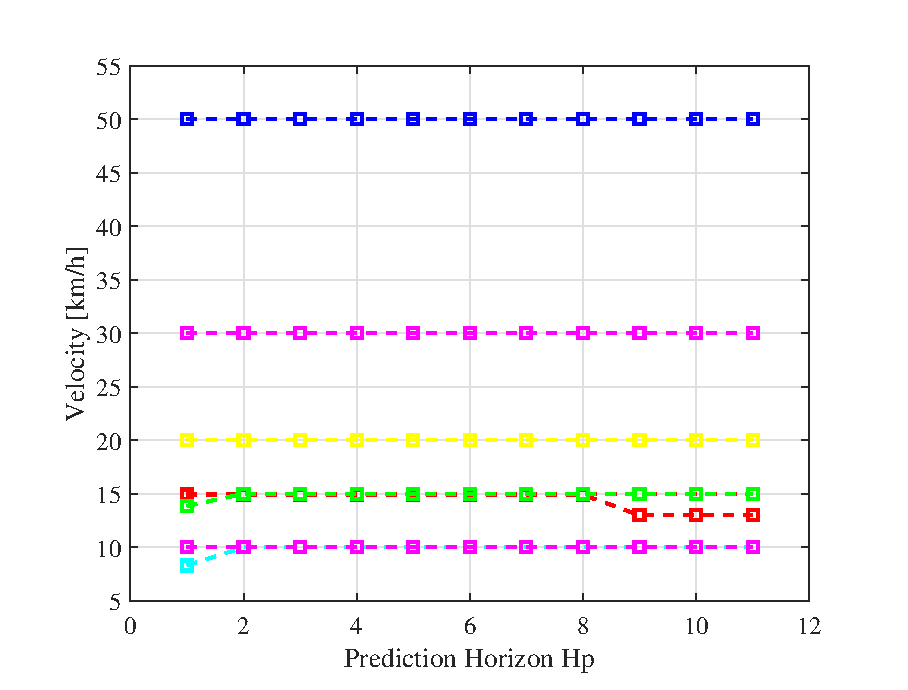
\includegraphics[width=\textwidth]{Kap6/red_lane/red_lane_vel10.eps}
    \caption{Predicted velocity profiles.}
    \label{fig:third_mpc10_redsce}
\end{subfigure}
\caption{MPC Iteration = 10. Lane reduction scenario}
\label{fig:figures}
\end{figure}
\\
Step 10 of the simulation in the reduced scenario shows how the vehicles have managed to occupy three lanes without colliding. In addition, fig  \ref{fig:first_mpc10_redsce} shows seven vehicles that have managed to occupy the central lane and five planning to occupy it. Moreover, it shows how they consider the speed, current position, and current lane to predict the future where they can enter lane three without colliding with the others.
\\

In fig \ref{fig:third_mpc10_redsce}, it is seen how most do not change their speed even though they may have different target speeds. This consensus is defined by the Game Theory Controller, where it is of greater importance to comply with the security regulations than to achieve the main objective for the controller.
\\



% .........................................
\begin{figure}[H]
\centering
\begin{subfigure}[t]{\textwidth}
    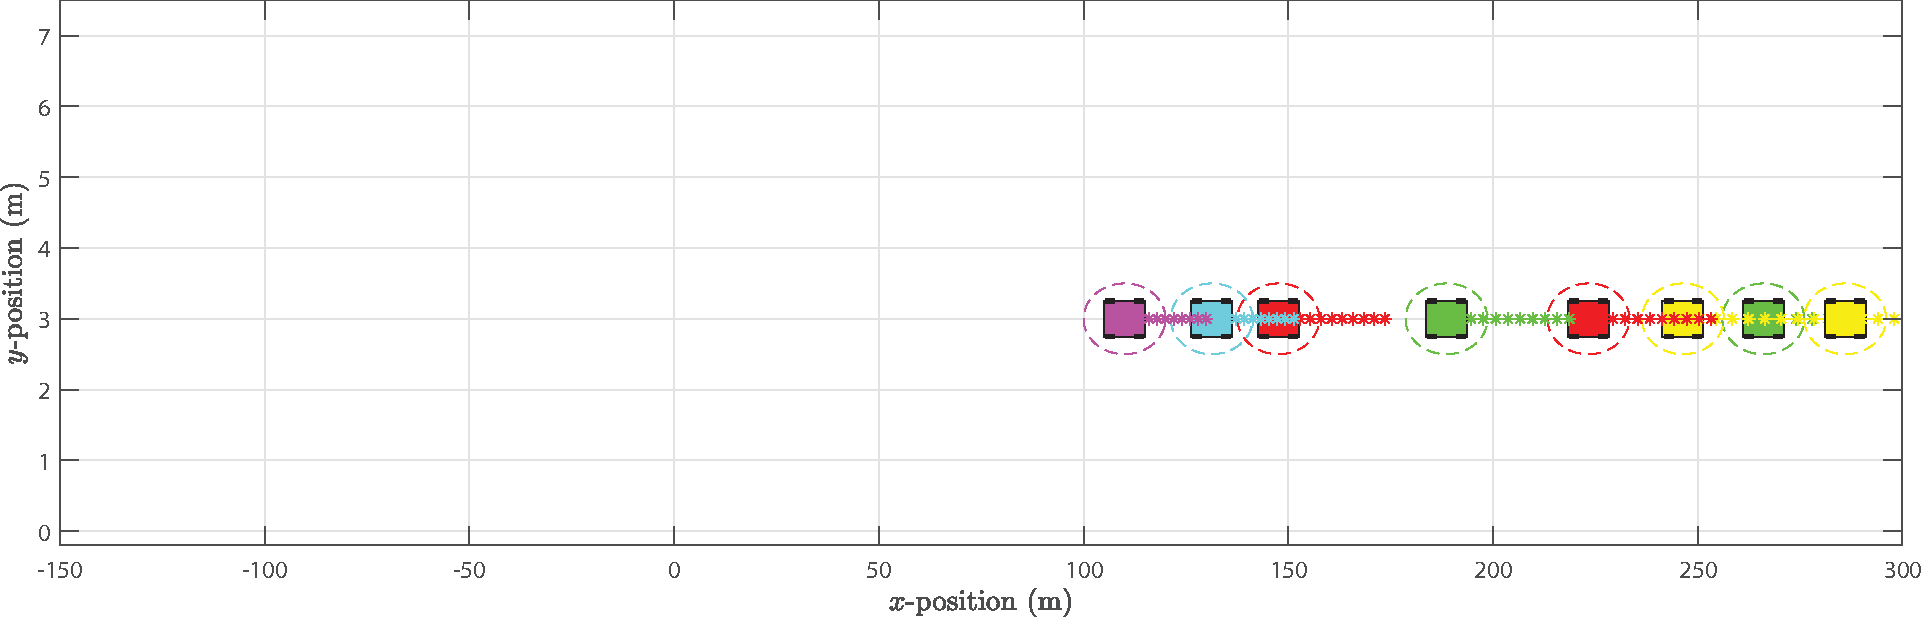
\includegraphics[width=\textwidth]{Kap6/red_lane/red_lane_traj36.eps}
    \caption{Predicted position at first position.}
    \label{fig:first}
\end{subfigure}
\vspace{1cm}
\begin{subfigure}[b]{0.45\textwidth}
    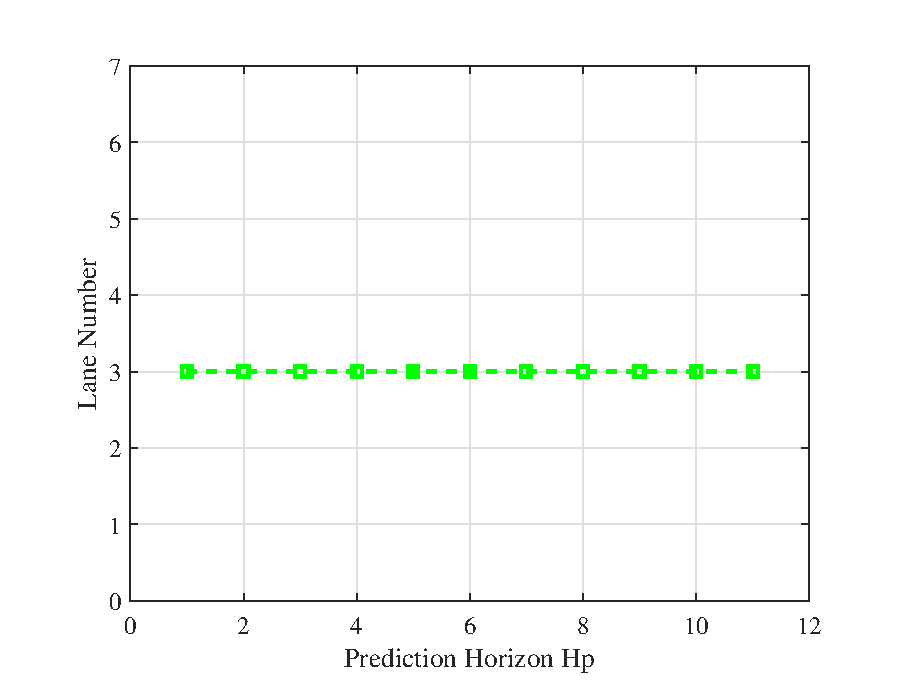
\includegraphics[width=\textwidth]{Kap6/red_lane/red_lane_lane36.eps}
    \caption{Predicted lane positions.}
    \label{fig:second}
\end{subfigure}
\hfill
\begin{subfigure}[b]{0.45\textwidth}
    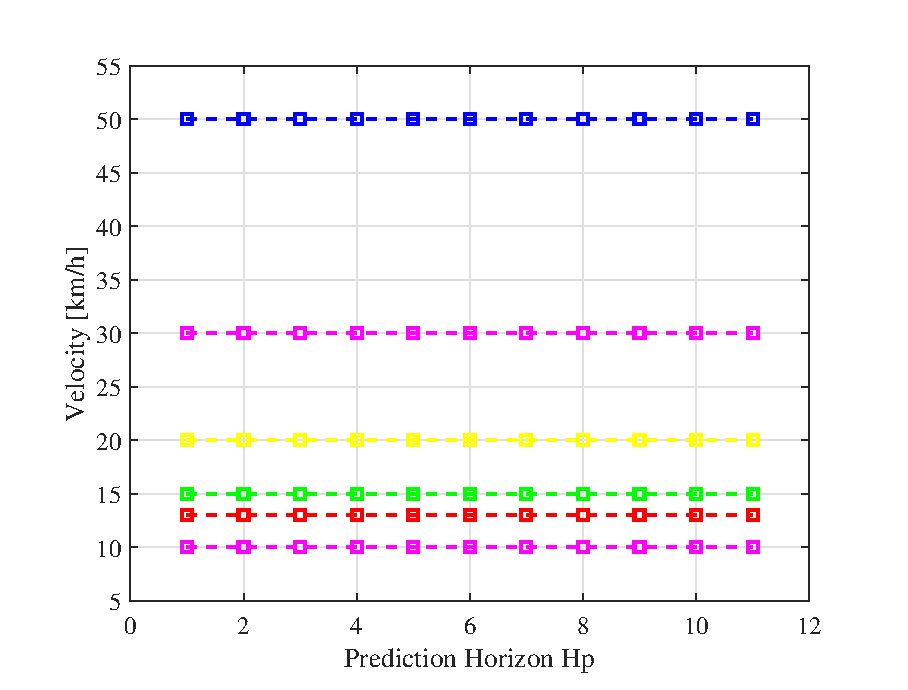
\includegraphics[width=\textwidth]{Kap6/red_lane/red_lane_vel36.eps}
    \caption{Predicted velocity profiles.}
    \label{fig:third}
\end{subfigure}
\caption{MPC Iteration = 30. Lane reduction scenario}
\label{fig:figures}
\end{figure}
% .......................................
\begin{figure}[H]
\centering
    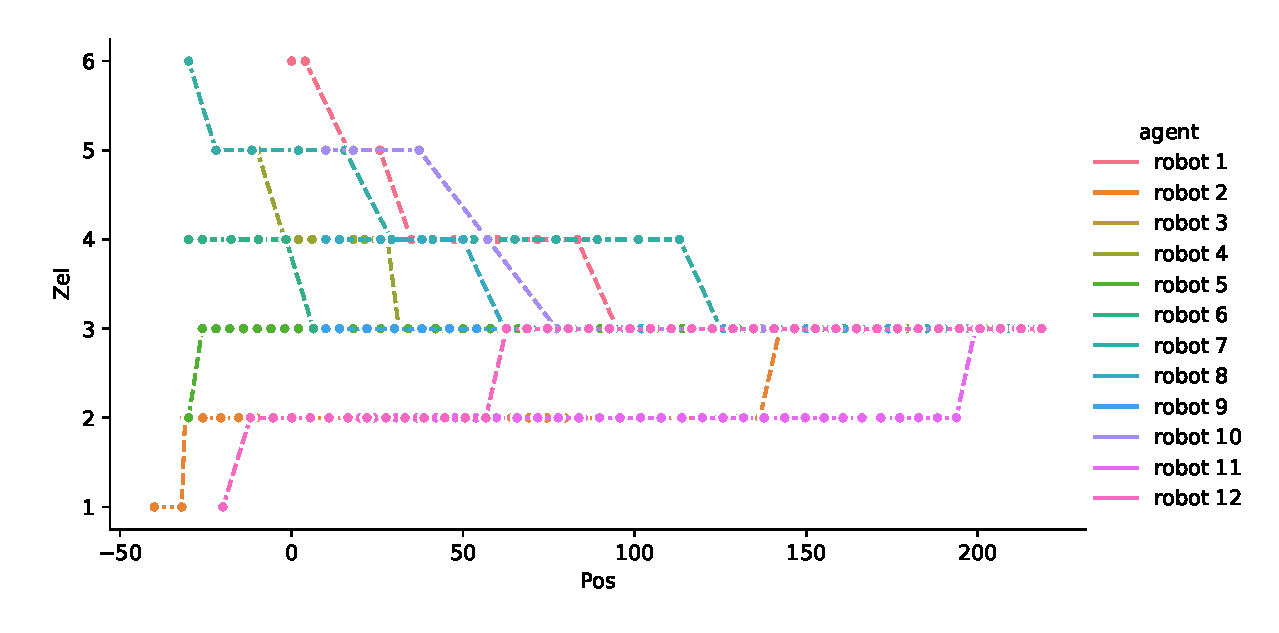
\includegraphics[width=0.8\textwidth]{Kap6/red_lane/red_lane_trajectories.eps}
    \caption{Trajectories of the entire network during the simulation time.}
    \label{red_lane_traject}
\end{figure}


Fig \ref{red_lane_traject} shows the trajectories travelled by vehicles as a result of a Generalized Potential Game control repeatedly solved by D-MPC for 12 vehicles. It is interesting to see how, despite the short space and time, 12 vehicles manage to synchronize to be able to enter the same lane without colliding and taking into account the decisions of the others. Also, the last vehicle $i=12$, is the last one that manages to join the lane. This is due to the initial conditions.

% ////////////////////////////

% {\color{blue} explicacion de como varian los tiempos de computo en cada iteracion  }

\begin{figure}[H]
\centering
    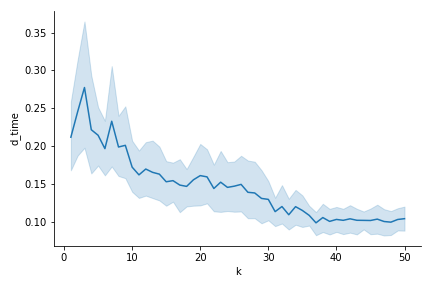
\includegraphics[width=.6\textwidth]{Kap6/red_lane/red_lane_d_time.png}
    \caption{Step Time}
    \label{red_lane_step_time}
\end{figure}

Figure \ref{red_lane_step_time} shows how the average solution time of the D-MPC is reduced by the reduction of restrictions and by the limited solution space. The network is at its maximum computation level at the simulation's beginning. This is due to the beginning, exist 12 vehicles trying to synchronize in order to be all on the same line.


\begin{figure}[H]
\centering
    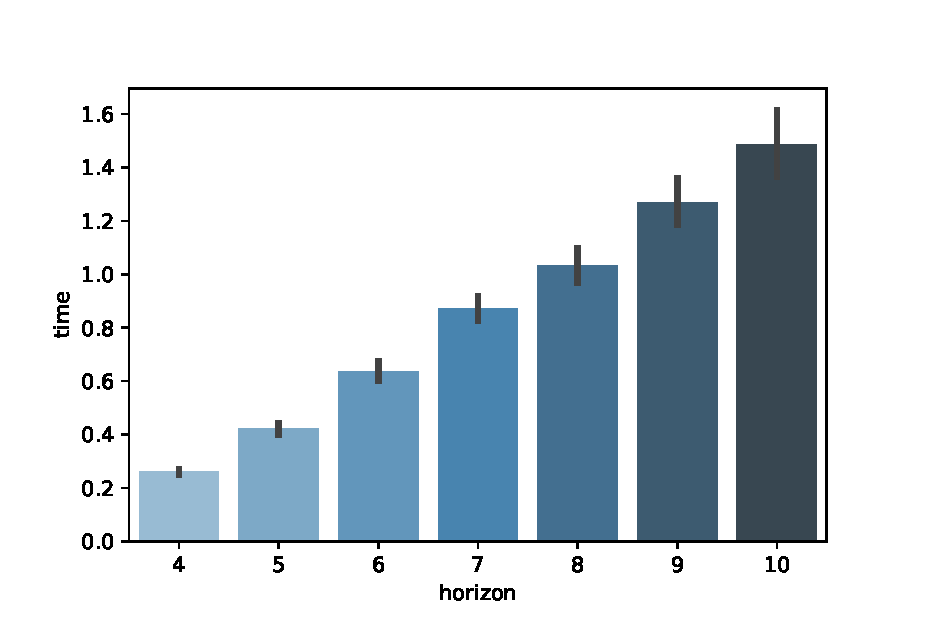
\includegraphics[width=0.6\textwidth]{Kap6/red_lane/red_lane_horizon_time.eps}
    \caption{Non-linear model of a differential robot.}
    \label{red_lane_horizon}
\end{figure}

The same feasibility analysis was performed by increasing the prediction horizon, and the D-MPC was able to solve the OCP without problems, Fig \ref{red_lane_horizon}. This system does not represent an effort to the Generalized Potential games theorem due to its low level of interactions between vehicles at the end of the simulation.




\begin{figure}[H]
\centering
    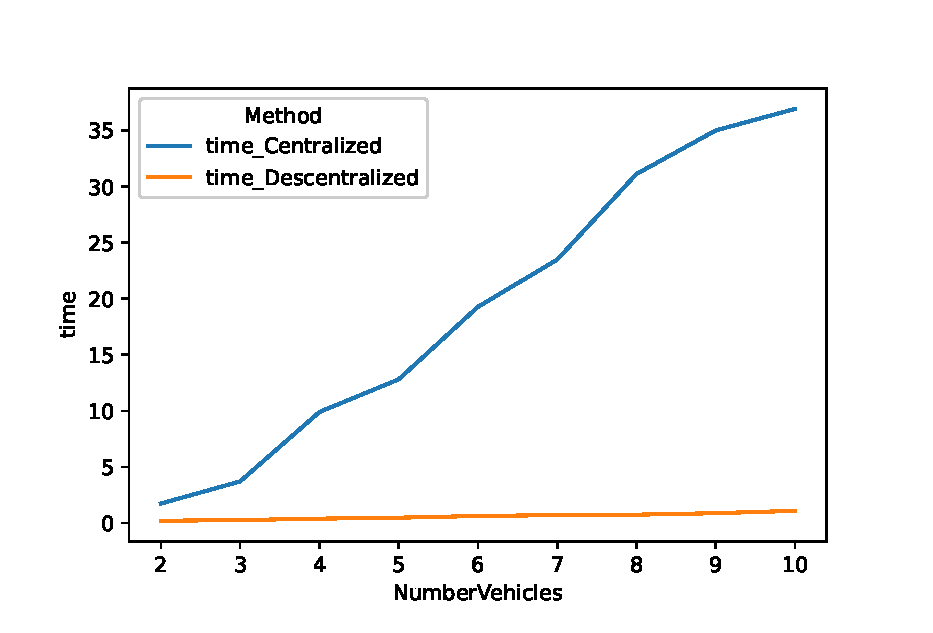
\includegraphics[width=0.6\textwidth]{Kap6/red_lane/red_lane_n_vehicles.eps}

\end{figure}

Finally, in the comparison of the times of each of the architectures, the C-MPC has an exponential increase in its solution time. The reduction of interactions does not significantly favor the centralized architecture. However, the D-MPC manages to maintain the average time of the complete simulation regardless of the increase in vehicles. This is due to the fact that the $\epsilon$-Nash equilibrium can be solved more quickly, and the OCP problem is reduced to the interaction of each vehicle with the vehicle in front and behind.

\subsection{Conclusion Reduced Scenario}

One of the scenarios that a vehicle could face on a highway would be that of construction on the road. This new change in the road conditions would be reflected in the set of spatial variables $\mathcal{L}$, which would be reduced from 6 to 1. We trust that the GMIPG in a D-MPC architecture shown in this thesis document can deal with this problem.
\\

\\
In C-MPC, when vehicles are merging into a single lane, it is difficult for them to find an optimal decision to avoid colliding with each other. With an increase in the prediction horizon, this inconvenience could be solved. However, it is not what was expected.
In D-MPC, the solution was always possible regardless of the prediction horizon used. In addition, the solution time could be reduced as each of the vehicles adhered to the single lane. This is because there are fewer connections that each agent must take into account to provide an optimal solution.
\\

In short, the C-MPC fails to give an adequate response to the problem of driving on a freeway with a lane reduction and in front of selfish agents trying to join the same lane. However, the D-MPC controller manages to deal with this problem with improved solution time and does not have problems with the solutions. See fig \ref{red_lane_step_time} .
The reduced scenario was chosen to analyze the behavior of both drivers in the face of a sudden reduction, such as the lanes of a highway. See fig \ref{red_lane_traject}. All vehicles manage to synchronize to be able to stay in a single lane.
